



Optimization is the art of doing the best you can with what you have got. Almost every quantitative question you might ask about the world -- how should a factory allocate its raw materials, how should goods be routed through a road network, how should two adversaries play a game -- can be phrased as the problem of making some function as small (or as large) as possible, subject to a list of constraints on what you are allowed to do. The subject is about turning that vague desire into a precise mathematical problem, and then actually \emph{solving} it.

Two themes run through everything we do. The first is \emph{convexity}: for a convex problem, local information is global information, and this is what makes optimization tractable at all. The second is \emph{duality}: every optimization problem casts a shadow, a second problem whose solution certifies the optimality of the first. Duality is what lets us know when we are done, and it appears in different disguises as complementary slackness, as shadow prices, as the max-flow min-cut theorem and as the minimax theorem of game theory. Along the way we will develop honest algorithms -- gradient descent, the simplex method, the transportation algorithm, Ford--Fulkerson -- that can be run by hand or by machine.

This article constitutes my notes for the `Optimization' course, held in Easter 2021 at Cambridge. These notes are \emph{not a transcription of the lectures}, and differ significantly in quite a few areas. Still, all lectured material should be covered.



\section{Convex Optimization}

\subsection{Optimization Problems}

In this course, we care about problems that look like `minimize $f(x)$ subject to $x \in X$', or problems with constraints that look like `minimize\footnote{We will almost always talk about minimizing, since maximizing is basically the same thing: to maximize $f$ we can minimize $-f$.} $f(x)$ subject to $x \in X$ where $h(x) = b$'.

In such problems, we call $f$ the \vocab{objective function}, and if $x \in \R^n$, we call the components \vocab{decision variables}. Constraints such as the one above can be given as a \vocab{functional constraint} $h(x) = b$ and a \vocab{regional constraint} $x \in X$. If both of the constraints hold for a given $x$, we say it is in the \vocab{feasible set} $X(b)$. A problem is feasible if the feasible set is non-empty, and bounded if the minimum over this set is bounded.

A point $x^* \in X(b)$ is \vocab{optimal} if it minimizes $f$ over $X(b)$. The value $f(x^*)$ is the \vocab{optimal cost}.

It is worth setting up some notation for all of this, since we are going to be writing down an awful lot of optimization problems. We will write a problem in the form
\begin{alignat*}{2}
    & \text{minimize} \quad && f(x) \\
    & \text{subject to} \quad && h(x) = b, \\
    & && x \in X,
\end{alignat*}
where $f : \R^n \rightarrow \R$, $h : \R^n \rightarrow \R^m$, $b \in \R^m$ and $X \subseteq \R^n$. So the feasible set is
$$
X(b) = \{x \in X : h(x) = b\}.
$$

\begin{remark}
    The split between `functional' and `regional' constraints is not intrinsic to the problem -- it is a choice that we make. The same set of feasible points can very often be described in several ways, and a large part of the skill in this course lies in choosing the description that makes the problem easiest to attack. Typically the regional constraint $x \in X$ will be something simple like $x \geq 0$ or $x \in \Z^n$, and the functional constraints will be the interesting ones that we handle with Lagrange multipliers.
\end{remark}

At first glance it looks as though we have restricted ourselves to \emph{equality} constraints, which would be a serious limitation. In fact we have not: an inequality constraint can always be converted into an equality constraint at the cost of introducing a new variable. If we want $h(x) \leq b$, we introduce a \vocab{slack variable} $s$ and write
$$
h(x) \leq b \quad \longleftrightarrow \quad h(x) + s = b, \quad s \geq 0.
$$
The new variable $s$ measures exactly how much `slack' there is in the constraint, and the sign condition $s \geq 0$ is pushed into the regional constraint. This trick will be used constantly.

\begin{example}
    Consider the problem of minimizing $x_1^2 + x_2^2$ subject to $x_1 + x_2 \geq 1$. Here $f(x) = x_1^2 + x_2^2$, and we can take $X = \R^2$ with the single functional constraint $x_1 + x_2 \geq 1$. Introducing a slack variable, this becomes: minimize $x_1^2 + x_2^2$ subject to $x_1 + x_2 - s = 1$ and $(x_1, x_2, s) \in \R^2 \times [0, \infty)$. The feasible set is a closed half-plane, and the optimum is at $x = (1/2, 1/2)$ with optimal cost $1/2$ -- the point of the half plane closest to the origin.
\end{example}

\subsection{Convex Functions}

We will first study optimization problems involving convex functions without constraints. In particular, we are going to study the problem:
\begin{center}
    Minimize $f(x)$, where $f : \R^n \rightarrow \R$ is a convex function.
\end{center}
The reason we will care specifically about convex functions is, as you will see, that local information about the function gives us global information about the function.

It is likely that you are already familiar with the notions of convex sets and convex functions.

\begin{definition}[Convex Set]
    A set $S \subseteq \R^n$ is \vocab{convex} if for all $x, y \in S$ and all $\lambda \in [0, 1]$ we have $\lambda x + (1 - \lambda) y \in S$.
\end{definition}

Informally, a set is convex if the line segment between any two points is totally contained in the set.

\begin{center}
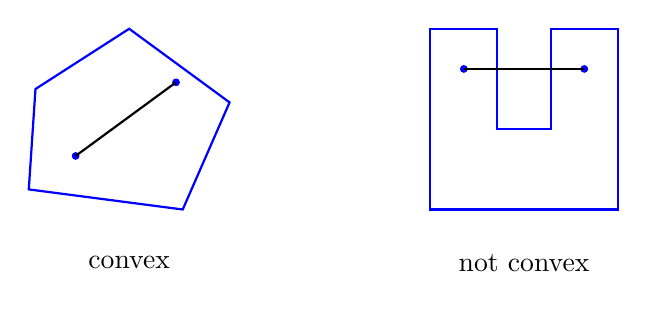
\begin{tikzpicture}[scale=0.85]
    \draw[thick, color=blue] (0,0) -- (2.3,-0.3) -- (3.0,1.3) -- (1.5,2.4) -- (0.1,1.5) -- cycle;
    \filldraw[color=blue] (0.7,0.5) circle (1.4pt);
    \filldraw[color=blue] (2.2,1.6) circle (1.4pt);
    \draw[thick] (0.7,0.5) -- (2.2,1.6);
    \node at (1.5,-1.1) {convex};

    \begin{scope}[xshift=6cm]
    \draw[thick, color=blue] (0,-0.3) -- (2.8,-0.3) -- (2.8,2.4) -- (1.8,2.4) -- (1.8,0.9) -- (1.0,0.9) -- (1.0,2.4) -- (0,2.4) -- cycle;
    \filldraw[color=blue] (0.5,1.8) circle (1.4pt);
    \filldraw[color=blue] (2.3,1.8) circle (1.4pt);
    \draw[thick] (0.5,1.8) -- (2.3,1.8);
    \node at (1.4,-1.1) {not convex};
    \end{scope}
\end{tikzpicture}
\end{center}

We can also define convexity for functions.

\begin{definition}[Convex Function]
    A function $f: S \rightarrow \R$ is \vocab{convex} if $S$ is convex and for all $x, y \in S$ and $\lambda \in [0, 1]$ we have
    $$
    f(\lambda x + (1 - \lambda) y) \leq \lambda f(x) + (1 - \lambda) f(y).
    $$
    If this inequality is strict (for $x \neq y$ and $\lambda \in (0,1)$) then the function is \vocab{strictly convex}. A function is called \vocab{concave} if $-f$ is convex.
\end{definition}

Again informally, this says that if we consider the graph of the function then the chord between two points will always lie above the function.

\begin{center}
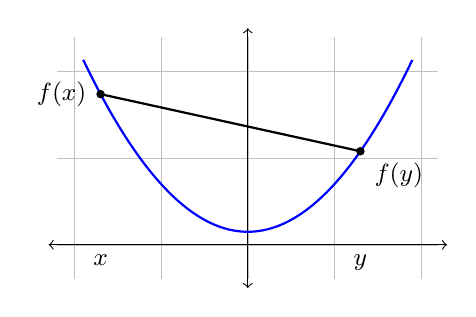
\begin{tikzpicture}[scale=1.1]
    \draw[ultra thin, color=lightgray] (-2.2,-0.4) grid (2.2,2.4);
    \draw[<->] (-2.3,0) -- (2.3,0);
    \draw[<->] (0,-0.5) -- (0,2.5);
    \draw[thick, samples=100, smooth, domain=-1.9:1.9, color=blue] plot (\x, {0.55*\x*\x + 0.15});
    \draw[thick] (-1.7,1.739) -- (1.3,1.0795);
    \filldraw (-1.7,1.739) circle (1.2pt);
    \filldraw (1.3,1.0795) circle (1.2pt);
    \node[anchor=east] at (-1.75,1.739) {\small $f(x)$};
    \node[anchor=north west] at (1.35,1.06) {\small $f(y)$};
    \node[anchor=north] at (-1.7,0) {\small $x$};
    \node[anchor=north] at (1.3,0) {\small $y$};
\end{tikzpicture}
\end{center}

Note that a linear function $f(x) = c \cdot x$ is both convex and concave, since the defining inequality holds with equality. So linear programming, which we will spend a lot of time on later, is a special case of convex optimization.

In general, checking the definition by hand is hard, and we typically use some other conditions to check for convexity.

\begin{proposition}[First-Order Conditions for Convexity]
A differentiable function $f: \R^n \rightarrow \R$ is convex if and only if for all $x, y \in \R^n$ we have
$$
f(y) \geq f(x) + (y - x) \cdot \nabla f(x).
$$
\end{proposition}
\begin{proof}
    We will first check that convexity implies that this condition holds by showing it holds for $n = 1$ and using that for the general case.

    If $f: \R \rightarrow \R$ is convex, and $x, y \in \R$ then for any $t \in (0, 1]$ we have
    \begin{align*}
        f((1 - t)x + ty) &= f(x + t(y - x)) \\
        & \leq (1 - t)f(x) + tf(y) \\
\implies f(y) & \geq f(x) + \frac{f(x + t(y - x)) - f(x)}{t}.
    \end{align*}
    Taking the limit as $t \rightarrow 0$, the quotient tends to $f'(x)(y - x)$, and so $f(y) \geq f(x) + f'(x)(y - x)$.

    Now for $f: \R^n \rightarrow \R$, taking any $x, y \in \R^n$ we can define the restricted function $g(t) = f((1 - t)x + ty)$. Since $f$ is convex, $g$ is also convex. We can then compute
    $$
    g'(t) = (y - x) \cdot \nabla f((1 - t) x + ty).
    $$
    So using the $n = 1$ case, we have $g(1) \geq g(0) + g'(0) (1 - 0)$, that is, $f(y) \geq f(x) + (y - x) \cdot \nabla f(x)$, so the condition holds as required.

    Now we will show that the first-order conditions imply convexity.
    For some $t \in [0, 1]$, we define $x_t = (1 - t) x + ty$. Then we know that
    \begin{align*}
        f(x) &\geq f(x_t) + (x - x_t) \cdot \nabla f(x_t), \\
        f(y) &\geq f(x_t) + (y - x_t) \cdot \nabla f(x_t).
    \end{align*}
    Multiplying the first by $(1 - t)$ and the second by $t$ and summing, the gradient terms combine to give
    $$
    (1-t)(x - x_t) + t(y - x_t) = (1-t)x + ty - x_t = 0,
    $$
    so we are left with
    $$
    (1 - t)f(x) + tf(y) \geq f(x_t),
    $$
    as required.
\end{proof}

This condition has a very clean geometric meaning: the tangent plane to the graph of $f$ at any point lies entirely \emph{below} the graph.

\begin{center}
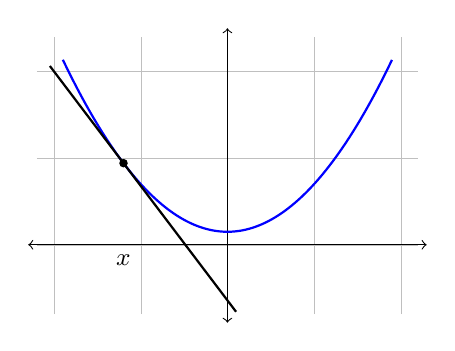
\begin{tikzpicture}[scale=1.1]
    \draw[ultra thin, color=lightgray] (-2.2,-0.8) grid (2.2,2.4);
    \draw[<->] (-2.3,0) -- (2.3,0);
    \draw[<->] (0,-0.9) -- (0,2.5);
    \draw[thick, samples=100, smooth, domain=-1.9:1.9, color=blue] plot (\x, {0.55*\x*\x + 0.15});
    % tangent at x = -1.2: f = 0.942, f' = -1.32
    \draw[thick, domain=-2.05:0.1] plot (\x, {0.942 - 1.32*(\x + 1.2)});
    \filldraw (-1.2,0.942) circle (1.2pt);
    \node[anchor=north] at (-1.2,0) {\small $x$};
\end{tikzpicture}
\end{center}

This picture makes the key fact about convex minimization obvious. If $\nabla f(x) = 0$ at some point $x$, then the first-order condition reads $f(y) \geq f(x)$ for \emph{all} $y$, so $x$ is a global minimum. In other words, for a convex function there is no such thing as a bad local minimum: every stationary point is a global minimum. This is exactly the promised phenomenon of local information giving global information, and it is the reason we can hope to minimize convex functions by walking downhill.

A possibly more familiar condition for convexity is the second-order condition. This involves the \emph{Hessian}, the generalization of the second derivative to $\R^n$.

\begin{definition}[Hessian]
    If $f: \R^n \rightarrow \R$ is a twice differentiable function, then the \vocab{Hessian matrix} $\nabla^2 f$ is the symmetric matrix of second derivatives given by
    $$
    (\nabla^2 f)_{ij} = \frac{\partial^2 f}{\partial x_i \partial x_j}.
    $$
\end{definition}

In particular, we care about a specific property of the Hessian matrix.

\begin{definition}[Positive Semidefinite]
    A symmetric matrix $A \in \R^{n \times n}$ is \vocab{positive semidefinite} if for all $x \in \R^n$ we have $x \cdot Ax \geq 0$; equivalently, if all of the eigenvalues of $A$ are non-negative. We write $A \succeq 0$. We write $A \succeq B$ to mean $A - B \succeq 0$.
\end{definition}

\begin{proposition}[Second-Order Conditions for Convexity]
A twice differentiable function $f:\R^n \rightarrow \R$ is convex if $\nabla^2 f(x)$ is positive semidefinite at all $x \in \R^n$.
\end{proposition}
\begin{proof}
    Using the Taylor expansion of $f$, we have
    $$
f(y) = f(x) + (y - x) \cdot \nabla f(x) + \frac{1}{2}(y - x) \cdot ( \nabla^2f(z)(y - x)),
    $$
    where $z = (1 - \lambda)x + \lambda y$ for some $\lambda \in [0, 1]$. Since $\nabla^2 f(z) \succeq 0$, the final term is non-negative, and so
    $$
    f(y) \geq f(x) + (y-x) \cdot \nabla f(x).
    $$
    Then by the first-order conditions, $f$ is convex.
\end{proof}

The converse also holds, but we will not need it.

\begin{example}
    Let us see the conditions in action.
    \begin{enumerate}[label=(\roman*)]
        \item $f(x) = x \cdot Ax$ for a symmetric matrix $A$ has $\nabla^2 f = 2A$, so $f$ is convex exactly when $A \succeq 0$.
        \item $f(x_1, x_2) = x_1^2 + 100 x_2^2$ has Hessian $\mathrm{diag}(2, 200) \succeq 0$, so is convex.
        \item $f(x) = e^{c \cdot x}$ has $\nabla^2 f = (cc^{T}) e^{c\cdot x}$, and $y \cdot (cc^T) y = (c \cdot y)^2 \geq 0$, so $f$ is convex for any $c$.
        \item $f(x_1, x_2) = x_1 x_2$ has Hessian $\begin{pmatrix} 0 & 1 \\ 1 & 0\end{pmatrix}$, whose eigenvalues are $\pm 1$. So this function is neither convex nor concave.
    \end{enumerate}
\end{example}

\subsection{Gradient Descent}

To solve our problem of minimizing $f(x)$ where $f : \R^n \rightarrow \R$ is a convex function, we can begin by noting that convexity implies that a local minimum is a global minimum. So if we find a point where the gradient of the function is $0$, then we would be finished. This suggests an extremely simple `greedy' strategy: start somewhere, look around for a nearby point with a smaller value of $f$, move there, and repeat.

To make this concrete we need to know which direction to move in. Taking a small step of size $\varepsilon$ in the direction $v$ and Taylor expanding,
$$
f(x + \varepsilon v) \approx f(x) + \varepsilon v \cdot \nabla f(x),
$$
so any $v$ with $v \cdot \nabla f(x) < 0$ will decrease $f$, at least for small enough $\varepsilon$. We call such a $v$ a \vocab{descent direction}. The most natural choice is $v = -\nabla f(x)$, which gives
$$
f(x - \varepsilon \nabla f(x)) \approx f(x) - \varepsilon \norm{\nabla f(x)}^2 \leq f(x).
$$

\begin{definition}[Gradient Descent]
    The \vocab{gradient descent} algorithm for minimizing $f$ is as follows.
    \begin{enumerate}[label=(\arabic*)]
        \item Choose a starting point $x_0$ and set $t = 0$.
        \item If $\nabla f(x_t) = 0$ (or we have run out of patience), stop and return $x_t$.
        \item Choose a step size $\eta_t > 0$ and set $x_{t + 1} = x_t - \eta_t \nabla f(x_t)$.
        \item Increment $t$ and go to (2).
    \end{enumerate}
\end{definition}

The whole art is in the choice of $\eta_t$. If it is too small we crawl; if it is too large we overshoot and oscillate. To say anything precise we need to control how fast the gradient can change.

\begin{definition}[Smoothness]
    A continuously differentiable $f : \R^n \rightarrow \R$ is \vocab{$\beta$-smooth} if $\nabla f$ is $\beta$-Lipschitz, that is
    $$
    \norm{\nabla f(x) - \nabla f(y)} \leq \beta \norm{x - y}
    $$
    for all $x, y$. If $f$ is twice differentiable this is equivalent to $\nabla^2 f(x) \preceq \beta I$ for all $x$.
\end{definition}

Smoothness says that the linear approximation to $f$ cannot be too badly wrong.

\begin{lemma}[Quadratic Upper Bound]
    If $f$ is $\beta$-smooth then for all $x, y$,
    $$
    f(y) \leq f(x) + (y - x) \cdot \nabla f(x) + \frac{\beta}{2} \norm{y - x}^2.
    $$
\end{lemma}
\begin{proof}
    By Taylor's theorem there is a point $z$ on the segment from $x$ to $y$ with
    $$
    f(y) = f(x) + (y-x)\cdot \nabla f(x) + \frac{1}{2}(y - x)\cdot (\nabla^2 f(z)(y-x)),
    $$
    and since $\nabla^2 f(z) \preceq \beta I$ we have $(y-x)\cdot (\nabla^2 f(z)(y-x)) \leq \beta \norm{y-x}^2$.
\end{proof}

Together with convexity this sandwiches $f$ between two functions that agree to first order at $x$: a linear lower bound and a quadratic upper bound. The quadratic upper bound is the useful one, because we can minimize it exactly.

\begin{corollary}
    If $f$ is $\beta$-smooth and we take a step of size $1/\beta$, then
    $$
    f\left(x - \frac{1}{\beta}\nabla f(x)\right) \leq f(x) - \frac{1}{2\beta}\norm{\nabla f(x)}^2.
    $$
\end{corollary}
\begin{proof}
    Minimizing the right-hand side of the quadratic upper bound over $y$, we differentiate to get $\nabla f(x) + \beta(y - x) = 0$, so the minimizer is $y = x - \frac{1}{\beta}\nabla f(x)$. Substituting this in,
    \begin{align*}
        f(y) &\leq f(x) - \frac{1}{\beta}\norm{\nabla f(x)}^2 + \frac{\beta}{2}\cdot \frac{1}{\beta^2}\norm{\nabla f(x)}^2 \\
        &= f(x) - \frac{1}{2\beta}\norm{\nabla f(x)}^2. \qedhere
    \end{align*}
\end{proof}

So each step makes definite progress, provided the gradient is not small. But a small gradient does not by itself mean we are near the optimum -- think of a function with a long, almost flat valley. To rule this out we need a lower bound on the curvature as well.

\begin{definition}[Strong Convexity]
    A function $f : \R^n \rightarrow \R$ is \vocab{$\alpha$-strongly convex} if for all $x, y$,
    $$
    f(y) \geq f(x) + (y - x)\cdot \nabla f(x) + \frac{\alpha}{2}\norm{y - x}^2.
    $$
    For twice differentiable $f$ this is equivalent to $\nabla^2 f(x) \succeq \alpha I$ for all $x$.
\end{definition}

\begin{lemma}
    Let $f$ be $\alpha$-strongly convex with minimum value $p^*$. Then for any $x$,
    $$
    p^* \geq f(x) - \frac{1}{2\alpha}\norm{\nabla f(x)}^2.
    $$
\end{lemma}
\begin{proof}
    Take the minimum over $y$ of both sides of the strong convexity inequality. The left-hand side becomes $p^*$. The right-hand side is a quadratic in $y$, minimized where $\nabla f(x) + \alpha(y - x) = 0$, that is at $y = x - \frac{1}{\alpha}\nabla f(x)$, giving
    $$
    p^* \geq f(x) - \frac{1}{\alpha}\norm{\nabla f(x)}^2 + \frac{1}{2\alpha}\norm{\nabla f(x)}^2 = f(x) - \frac{1}{2\alpha}\norm{\nabla f(x)}^2. \qedhere
    $$
\end{proof}

In other words, if $\norm{\nabla f(x)} \leq \sqrt{2\alpha\varepsilon}$ then $f(x) \leq p^* + \varepsilon$: for a strongly convex function, a small gradient really does mean we are nearly done. Putting the two bounds together gives a genuine convergence guarantee.

\begin{theorem}[Convergence of Gradient Descent]
    Let $f$ be $\beta$-smooth and $\alpha$-strongly convex with $0 < \alpha \leq \beta$, and let $x^*$ be its minimizer. Then gradient descent with step size $1/\beta$ satisfies
    $$
    f(x_T) - f(x^*) \leq \left(1 - \frac{\alpha}{\beta}\right)^T\left(f(x_0) - f(x^*)\right) \leq e^{-\alpha T/\beta}\cdot\frac{\beta}{2}\norm{x_0 - x^*}^2.
    $$
\end{theorem}
\begin{proof}
    Write $\delta_t = f(x_t) - f(x^*)$. By the corollary above and then the lemma above (applied at $x_t$, with $p^* = f(x^*)$),
    $$
    \delta_{t+1} \leq \delta_t - \frac{1}{2\beta}\norm{\nabla f(x_t)}^2 \leq \delta_t - \frac{\alpha}{\beta}\delta_t = \left(1 - \frac{\alpha}{\beta}\right)\delta_t,
    $$
    where the middle step used $\norm{\nabla f(x_t)}^2 \geq 2\alpha \delta_t$. Induction gives the first inequality, and $1 - u \leq e^{-u}$ gives the second. Finally, $\beta$-smoothness applied at $x^*$ (where $\nabla f(x^*) = 0$) gives $\delta_0 \leq \frac{\beta}{2}\norm{x_0 - x^*}^2$.
\end{proof}

The quantity $\kappa = \beta/\alpha \geq 1$ is called the \vocab{condition number} of $f$. To get $f(x_T) - f(x^*) \leq \varepsilon$ we need about $\kappa \log(1/\varepsilon)$ steps; each extra decimal place of accuracy costs a constant number of extra steps, which is called \emph{linear convergence} and is very fast indeed. But the constant is $\kappa$, and if $\kappa$ is huge then convergence is slow.

\begin{example}
    Consider $f(x_1, x_2) = \frac{1}{2}(x_1^2 + 100x_2^2)$, whose Hessian is $\mathrm{diag}(1, 100)$, so $\alpha = 1$, $\beta = 100$ and $\kappa = 100$. The level sets are extremely elongated ellipses, and the gradient at a typical point points almost straight at the long axis rather than at the origin. Gradient descent therefore zig-zags across the valley making very slow progress along it.
\end{example}

\begin{center}
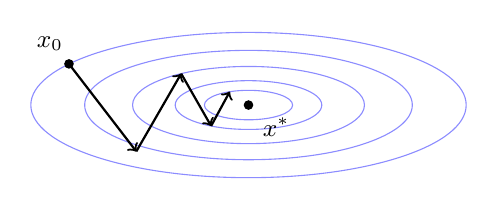
\begin{tikzpicture}[scale=0.95]
    \draw[color=blue!45] (0,0) ellipse (2.91 and 0.971);
    \draw[color=blue!45] (0,0) ellipse (2.19 and 0.731);
    \draw[color=blue!45] (0,0) ellipse (1.55 and 0.516);
    \draw[color=blue!45] (0,0) ellipse (0.98 and 0.326);
    \draw[color=blue!45] (0,0) ellipse (0.59 and 0.197);
    \draw[thick,->] (-2.4,0.55) -- (-1.5,-0.62);
    \draw[thick,->] (-1.5,-0.62) -- (-0.9,0.42);
    \draw[thick,->] (-0.9,0.42) -- (-0.5,-0.28);
    \draw[thick,->] (-0.5,-0.28) -- (-0.25,0.18);
    \filldraw (-2.4,0.55) circle (1.6pt);
    \node[anchor=south east] at (-2.35,0.6) {\small $x_0$};
    \filldraw (0,0) circle (1.6pt);
    \node[anchor=north west] at (0.06,-0.04) {\small $x^*$};
\end{tikzpicture}
\end{center}

\subsection{Newton's Method and Barrier Methods}

The problem in the example above is that gradient descent treats all coordinates the same way, whereas the function does not. The fix is to rescale by the Hessian. Recall that the second-order approximation to $f$ near $x_t$ is
$$
f(x) \approx f(x_t) + (x - x_t)\cdot \nabla f(x_t) + \frac{1}{2}(x - x_t) \cdot \left(\nabla^2 f(x_t)(x - x_t)\right),
$$
and minimizing the right-hand side over $x$ gives $x = x_t - (\nabla^2 f(x_t))^{-1}\nabla f(x_t)$.

\begin{definition}[Newton's Method]
    \vocab{Newton's method} is the iteration
    $$
    x_{t + 1} = x_t - \left(\nabla^2 f(x_t)\right)^{-1}\nabla f(x_t).
    $$
\end{definition}

So instead of approximating $f$ by a linear function and stepping a fixed distance, we approximate it by a paraboloid and jump straight to the bottom of that paraboloid. Near the optimum this converges quadratically: one can show that
$$
\norm{x_{t+1} - x^*} \leq c\norm{x_t - x^*}^2
$$
once $x_t$ is close enough to $x^*$, so the number of correct digits roughly doubles each step. The price is that we have to compute and invert an $n \times n$ matrix at every step.

\begin{remark}
    In one dimension, Newton's method reads $x_{t+1} = x_t - f'(x_t)/f''(x_t)$, which is exactly the familiar Newton--Raphson iteration for finding a root of $g = f'$. Minimizing $f$ and finding a zero of its derivative are of course the same problem.
\end{remark}

Finally, a word about constraints. Suppose we want to minimize $f(x)$ subject to $f_i(x) \leq 0$ for $i = 1, \dots, m$. We would love to reduce this to an unconstrained problem, and the obvious way is to minimize
$$
f(x) + \sum_{i = 1}^m \phi(f_i(x)),
$$
where $\phi(y) = 0$ for $y \leq 0$ and $\phi(y) = +\infty$ for $y > 0$. This is exactly the original problem, but $\phi$ is not remotely differentiable and so all of our machinery fails. Instead we use a smooth approximation.

\begin{definition}[Logarithmic Barrier]
    The \vocab{logarithmic barrier method} solves the unconstrained problem
    $$
    \text{minimize} \quad tf(x) - \sum_{i = 1}^m \log(-f_i(x))
    $$
    for a sequence of increasing values of $t > 0$, using the previous solution as the starting point for the next.
\end{definition}

The function $-\log(-y)$ is $+\infty$ for $y \geq 0$ and finite for $y < 0$, rising steeply as $y \rightarrow 0^-$; it fences the iterates inside the feasible region. As $t \rightarrow \infty$ the objective $f$ dominates the barrier, and the minimizer converges to the solution of the constrained problem. Each subproblem is solved by Newton's method. This is the basic idea behind \emph{interior point methods}, which are what modern solvers actually use.

\section{Lagrangian Methods}

Everything in the previous section was about \emph{unconstrained} problems. Real problems come with constraints, and the central idea for handling them -- one of the great ideas in the subject -- is to not handle them at all. Instead we build the constraints into the objective function with a price attached, and then solve an unconstrained problem. If we get the prices right, the solution of the unconstrained problem automatically satisfies the constraints.

\subsection{The Lagrangian}

Throughout this section we consider the problem
\begin{alignat*}{2}
    & \text{minimize} \quad && f(x) \\
    & \text{subject to} \quad && h(x) = b, \\
    & && x \in X,
\end{alignat*}
where $h : \R^n \rightarrow \R^m$. We will refer to this as the \vocab{primal problem}, denoted $(P)$.

\begin{definition}[Lagrangian]
    The \vocab{Lagrangian} of the problem $(P)$ is the function
    $$
    L(x, \lambda) = f(x) - \lambda \cdot (h(x) - b),
    $$
    where $\lambda \in \R^m$ is the vector of \vocab{Lagrange multipliers}.
\end{definition}

The point is this. If $x$ satisfies the functional constraint $h(x) = b$, then the second term vanishes and $L(x, \lambda) = f(x)$, whatever $\lambda$ is. So on the feasible set the Lagrangian \emph{is} the objective function. Off the feasible set, the term $-\lambda \cdot (h(x) - b)$ acts as a penalty (or a reward, depending on signs) for violating the constraints, and if we choose $\lambda$ well then the penalty is enough to keep the unconstrained minimizer of $L$ inside the feasible set. Making this precise gives the following theorem, which will be our main tool.

\begin{theorem}[Lagrangian Sufficiency]
    Suppose we can find $\lambda^* \in \R^m$ and $x^* \in X$ such that
    \begin{enumerate}[label=(\roman*)]
        \item $x^*$ minimizes $L(\cdot, \lambda^*)$ over all of $X$, that is, $L(x^*, \lambda^*) = \min_{x \in X} L(x, \lambda^*)$; and
        \item $x^*$ is feasible, that is, $x^* \in X(b)$.
    \end{enumerate}
    Then $x^*$ is optimal for $(P)$.
\end{theorem}
\begin{proof}
    Since $x^*$ is feasible we certainly have $f(x^*) \geq \min_{x \in X(b)}f(x)$, so we only need the reverse inequality. For this, note that if $x \in X(b)$ then $h(x) - b = 0$, so subtracting $\lambda^* \cdot (h(x) - b)$ changes nothing:
    \begin{align*}
        \min_{x \in X(b)}f(x) &= \min_{x \in X(b)}\left(f(x) - \lambda^*\cdot(h(x) - b)\right)\\
        &\geq \min_{x \in X}\left(f(x) - \lambda^*\cdot(h(x) - b)\right) \\
        &= \min_{x \in X}L(x, \lambda^*) \\
        &= L(x^*, \lambda^*) \\
        &= f(x^*) - \lambda^* \cdot (h(x^*) - b) = f(x^*).
    \end{align*}
    Here the inequality is because we are minimizing over a larger set $X \supseteq X(b)$, the next-to-last line is hypothesis (i), and the last line is hypothesis (ii). So $f(x^*) = \min_{x \in X(b)}f(x)$ as claimed.
\end{proof}

This gives us a recipe. Rather than minimize over the awkward set $X(b)$, we minimize over the nice set $X$ for each fixed $\lambda$, obtaining a candidate $x^*(\lambda)$, and then hunt for the value of $\lambda$ making $x^*(\lambda)$ feasible. Notice that we have to be careful: for some $\lambda$ the Lagrangian will not have a finite minimum at all. So we define
$$
\Lambda = \left\{\lambda \in \R^m : \inf_{x \in X}L(x, \lambda) > -\infty\right\},
$$
and only consider $\lambda \in \Lambda$.

\begin{example}
    Consider the problem
    \begin{alignat*}{2}
        & \text{minimize} \quad && -x_1 - x_2 + x_3 \\
        & \text{subject to} \quad && x_1^2 + x_2^2 = 4, \\
        & && x_1 + x_2 + x_3 = 1,
    \end{alignat*}
    over $x \in \R^3$. So $X = \R^3$ and $b = (4, 1)$. The Lagrangian is
    \begin{align*}
        L(x, \lambda) &= -x_1 - x_2 + x_3 - \lambda_1(x_1^2 + x_2^2 - 4) - \lambda_2(x_1 + x_2 + x_3 - 1)\\
        &= \left(-(1 + \lambda_2)x_1 - \lambda_1 x_1^2\right) + \left(-(1 + \lambda_2)x_2 - \lambda_1 x_2^2\right) + (1 - \lambda_2)x_3 + 4\lambda_1 + \lambda_2.
    \end{align*}
    We have arranged the terms so that each variable appears in exactly one bracket, and so we can minimize each bracket separately.

    First, which $\lambda$ lie in $\Lambda$? The $x_3$ term is linear, so unless $\lambda_2 = 1$ we can send it to $-\infty$. The $x_1$ term is a quadratic with leading coefficient $-\lambda_1$, so we need $\lambda_1 \leq 0$; and if $\lambda_1 = 0$ then the remaining linear term $-(1 + \lambda_2)x_1 = -2x_1$ is unbounded below. So $\Lambda = \{\lambda : \lambda_1 < 0, \lambda_2 = 1\}$.

    For such $\lambda$, minimizing each bracket by differentiating,
    $$
    -(1 + \lambda_2) - 2\lambda_1 x_1 = 0 \implies x_1 = \frac{-2}{2\lambda_1} = \frac{-1}{\lambda_1},
    $$
    and identically $x_2 = -1/\lambda_1$. Note $x_3$ is completely free (its coefficient is zero), which is exactly what we want -- it leaves us room to satisfy the second constraint.

    Now we impose feasibility. From $x_1^2 + x_2^2 = 4$ we get $2/\lambda_1^2 = 2$, so $\lambda_1 = -1/\sqrt{2}$ (taking the negative root as required) and $x_1 = x_2 = \sqrt{2}$. Then the second constraint gives $x_3 = 1 - 2\sqrt{2}$.

    By Lagrangian sufficiency, $x^* = (\sqrt 2, \sqrt2, 1 - 2\sqrt 2)$ is optimal, with optimal cost $-1 - 2\sqrt 2$.
\end{example}

\subsection{Inequality Constraints and Complementary Slackness}

Now suppose the constraints are inequalities:
\begin{alignat*}{2}
    & \text{minimize} \quad && f(x) \\
    & \text{subject to} \quad && h(x) \leq b, \\
    & && x \in X.
\end{alignat*}
We already know how to deal with this -- add a slack variable $s \geq 0$ and write $h(x) + s = b$. The Lagrangian becomes
$$
L(x, s, \lambda) = f(x) - \lambda \cdot (h(x) + s - b),
$$
and we now minimize over $x \in X$ and $s \geq 0$. Writing the Lagrangian as
$$
L(x, s, \lambda) = \underbrace{f(x) - \lambda\cdot(h(x) - b)}_{\text{does not involve }s} - \lambda \cdot s,
$$
we can read off two things immediately.

Firstly, since $s$ ranges over all of $[0, \infty)^m$, the term $-\lambda \cdot s$ is bounded below only if $\lambda \leq 0$. So $\lambda \in \Lambda$ forces $\lambda \leq 0$: with the sign convention above, \emph{Lagrange multipliers for $\leq$ constraints are non-positive}.

Secondly, given $\lambda \leq 0$, the minimum over $s \geq 0$ of $-\lambda\cdot s$ is attained by taking $s_i = 0$ whenever $\lambda_i < 0$ (and $s_i$ arbitrary when $\lambda_i = 0$). In either case the minimizing $s$ satisfies $\lambda_i s_i = 0$ for every $i$. This is important enough to have a name.

\begin{theorem}[Complementary Slackness]
    At an optimum obtained by the Lagrangian method, for each $i$ we have
    $$
    \lambda_i s_i = 0, \quad\text{ equivalently }\quad \lambda_i\left(h_i(x) - b_i\right) = 0.
    $$
    So for each $i$, either the constraint is \vocab{tight} ($h_i(x) = b_i$) or the multiplier vanishes ($\lambda_i = 0$) -- or both.
\end{theorem}

In words: a constraint that is not binding has zero multiplier. If we are not up against a constraint, then it is not costing us anything, so its price should be zero. We will see this interpretation made precise in a moment, and we will meet the same phenomenon again and again -- in linear programming, in the transportation algorithm, and in game theory.

Complementary slackness is enormously useful in practice, because it lets us split into cases: for each constraint, either $s_i = 0$ or $\lambda_i = 0$, and often most of the cases can be eliminated quickly.

\begin{example}
    Consider
    \begin{alignat*}{2}
        & \text{minimize} \quad && x_1 - 3x_2 \\
        & \text{subject to} \quad && x_1^2 + x_2^2 \leq 4, \\
        & && x_1 + x_2 \leq 2,
    \end{alignat*}
    over $x \in \R^2$. Adding slack variables $s_1, s_2 \geq 0$, the Lagrangian is
    \begin{align*}
        L &= (x_1 - 3x_2) - \lambda_1(x_1^2 + x_2^2 + s_1 - 4) - \lambda_2(x_1 + x_2 + s_2 - 2)\\
        &= \left((1 - \lambda_2)x_1 - \lambda_1x_1^2\right) + \left((-3 - \lambda_2)x_2 - \lambda_1 x_2^2\right) - \lambda_1 s_1 - \lambda_2 s_2 + 4\lambda_1 + 2\lambda_2.
    \end{align*}
    As discussed, $\lambda_1, \lambda_2 \leq 0$. Minimizing the two brackets,
    $$
    (1 - \lambda_2) - 2\lambda_1 x_1 = 0, \qquad (-3 - \lambda_2) - 2\lambda_1 x_2 = 0.
    $$
    If $\lambda_1 = 0$ these read $\lambda_2 = 1$ and $\lambda_2 = -3$, which is a contradiction. So $\lambda_1 < 0$, and complementary slackness gives $s_1 = 0$, i.e.\ the first constraint is tight: $x_1^2 + x_2^2 = 4$.

    Now suppose $\lambda_2 < 0$. Then $s_2 = 0$ too, so $x_1 + x_2 = 2$ as well. Combined with $x_1^2 + x_2^2 = 4$ this gives $(x_1, x_2) = (0,2)$ or $(2,0)$. Substituting into the two stationarity equations, the first case gives $(\lambda_1, \lambda_2) = (1, -3)$ and the second gives $(\lambda_1, \lambda_2) = (-1, 1)$; both have a positive multiplier, so both are impossible.

    Hence $\lambda_2 = 0$, and the stationarity equations become $x_1 = 1/(2\lambda_1)$ and $x_2 = -3/(2\lambda_1)$. Substituting into $x_1^2 + x_2^2 = 4$,
    $$
    \frac{1 + 9}{4\lambda_1^2} = 4 \implies \lambda_1^2 = \frac{5}{8} \implies \lambda_1 = -\sqrt{5/8},
    $$
    giving
    $$
    (x_1, x_2) = \left(-\sqrt{2/5},\ 3\sqrt{2/5}\right).
    $$
    Finally we check that this is feasible for the second constraint: $x_1 + x_2 = 2\sqrt{2/5} \approx 1.26 \leq 2$, so $s_2 = 2 - 2\sqrt{2/5} \geq 0$. By Lagrangian sufficiency this is optimal, with cost $-10\sqrt{2/5} = -2\sqrt{10}$.
\end{example}

Let us record the general procedure, since it is what we will do every time.

\begin{remark}[The Lagrangian Recipe]
    To solve `minimize $f(x)$ subject to $h(x) \leq b$, $x \in X$':
    \begin{enumerate}[label=(\arabic*)]
        \item Introduce slack variables to get equality constraints $h(x) + s = b$, $s \geq 0$.
        \item Form the Lagrangian $L(x, s, \lambda) = f(x) - \lambda\cdot(h(x) + s - b)$.
        \item Find $\Lambda$, the set of $\lambda$ for which $\inf_{x \in X, s \geq 0}L$ is finite.
        \item For each $\lambda \in \Lambda$, find the minimizers $x^*(\lambda), s^*(\lambda)$.
        \item Find $\lambda^* \in \Lambda$ for which $x^*(\lambda^*), s^*(\lambda^*)$ is feasible. Then $x^*(\lambda^*)$ is optimal.
    \end{enumerate}
\end{remark}

\subsection{Lagrangian Duality}

The Lagrangian recipe raises an obvious worry: what if there is no $\lambda^*$ that makes the minimizer feasible? Then the method fails, and we would like to understand when and why. The answer is the theory of duality, which is much more than a diagnostic tool -- it is arguably the most important structure in the whole subject.

\begin{definition}[Dual Function and Dual Problem]
    The \vocab{dual function} associated with $(P)$ is
    $$
    g(\lambda) = \inf_{x \in X}L(x, \lambda),
    $$
    defined for $\lambda \in \Lambda$. The \vocab{dual problem} $(D)$ is
    \begin{alignat*}{2}
        & \text{maximize} \quad && g(\lambda) \\
        & \text{subject to} \quad && \lambda \in \Lambda.
    \end{alignat*}
\end{definition}

Note that $g$ is an infimum of \emph{affine} functions of $\lambda$ (one for each $x$), and an infimum of affine functions is always concave. So the dual problem is always the maximization of a concave function over a convex set, i.e.\ always a convex problem, no matter how horrible the primal problem was. This is remarkable and is one reason duality is so useful.

\begin{theorem}[Weak Duality]
    If $x \in X(b)$ and $\lambda \in \Lambda$, then $f(x) \geq g(\lambda)$. In particular
    $$
    \inf_{x \in X(b)}f(x) \geq \sup_{\lambda \in \Lambda}g(\lambda).
    $$
\end{theorem}
\begin{proof}
    This is the first two lines of the proof of Lagrangian sufficiency. For $x \in X(b)$ we have $h(x) = b$, so
    $$
    f(x) = f(x) - \lambda\cdot(h(x) - b) = L(x, \lambda) \geq \inf_{x' \in X}L(x', \lambda) = g(\lambda). \qedhere
    $$
\end{proof}

So every feasible $\lambda$ gives a \emph{lower bound} on the optimal cost, and every feasible $x$ gives an \emph{upper bound}. This is already valuable: if we find $x$ and $\lambda$ with $f(x) = g(\lambda)$, we have proved that both are optimal without any further work. In general, though, there may be a gap.

\begin{definition}[Duality Gap]
    The \vocab{duality gap} is
    $$
    \inf_{x \in X(b)}f(x) - \sup_{\lambda \in \Lambda}g(\lambda) \geq 0.
    $$
    If the duality gap is zero we say that \vocab{strong duality} holds.
\end{definition}

The relationship with the Lagrangian method is exactly what one would hope.

\begin{proposition}
    The Lagrangian method succeeds -- that is, there is a $\lambda^*$ whose associated minimizer is feasible -- if and only if strong duality holds.
\end{proposition}
\begin{proof}
    If the method succeeds with multiplier $\lambda^*$ and minimizer $x^*$, then by the proof of Lagrangian sufficiency, $g(\lambda^*) = L(x^*, \lambda^*) = f(x^*) = \min_{x \in X(b)}f(x)$, so the gap is zero.

    Conversely if the gap is zero then there is $\lambda^*$ (or a sequence approaching it) with $g(\lambda^*) = \inf_{x \in X(b)}f(x)$, and the chain of inequalities in the sufficiency proof collapses to equalities, so the minimizer of $L(\cdot, \lambda^*)$ is feasible and optimal.
\end{proof}

So we should ask: when does strong duality hold? The answer is beautifully geometric.

\subsection{Supporting Hyperplanes}

The key object is the following.

\begin{definition}[Value Function]
    The \vocab{value function} of the problem $(P)$ is $\phi : \R^m \rightarrow \R \cup \{\pm\infty\}$ given by
    $$
    \phi(c) = \inf_{x \in X(c)}f(x),
    $$
    the optimal cost when the right-hand side of the functional constraint is changed from $b$ to $c$.
\end{definition}

So $\phi(b)$ is the number we are trying to compute, and $\phi$ tells us how that number responds to perturbing the constraints. Now here is the definition that makes everything work.

\begin{definition}[Supporting Hyperplane]
    A function $\phi : \R^m \rightarrow \R$ has a \vocab{supporting hyperplane} at $b$ if there is some $\lambda \in \R^m$ such that
    $$
    \phi(c) \geq \phi(b) + \lambda\cdot(c - b) \quad\text{ for all } c \in \R^m.
    $$
\end{definition}

That is, there is a hyperplane through the point $(b, \phi(b))$ which lies entirely below the graph of $\phi$. Compare this with the first-order condition for convexity, where the tangent plane at every point lies below the graph. Indeed one can show (we will not prove it) that $\phi$ is convex if and only if $\phi$ has a supporting hyperplane at every point.

\begin{center}
\begin{tikzpicture}[scale=1.0]
    \draw[<->] (-0.4,0) -- (5.2,0) node[anchor=north] {\small $c$};
    \draw[<->] (0,-0.4) -- (0,3.4) node[anchor=east] {\small $\phi$};
    \draw[thick, samples=100, smooth, domain=0.35:4.75, color=blue] plot (\x, {0.32*(\x-2.6)*(\x-2.6) + 0.7});
    % supporting hyperplane at b = 3.4: phi = 0.9048, slope = 0.64*(0.8)=0.512
    \draw[thick] (1.8,0.085) -- (4.6,1.519);
    \filldraw (3.4,0.9048) circle (1.4pt);
    \draw[dashed] (3.4,0) -- (3.4,0.9048);
    \node[anchor=north] at (3.4,0) {\small $b$};
    \node[anchor=north west] at (4.6,1.519) {\small slope $\lambda$};
    \node[anchor=south east, color=blue] at (4.8,2.12) {\small $\phi$};
\end{tikzpicture}
\end{center}

\begin{theorem}[Strong Duality]
    Strong duality holds for $(P)$ if and only if the value function $\phi$ has a supporting hyperplane at $b$.
\end{theorem}
\begin{proof}
    Suppose first that $\phi$ has a supporting hyperplane at $b$, with normal given by $\lambda$. The trick is to compute $g(\lambda)$ by splitting the minimization over $x \in X$ into a minimization over the possible values $c = h(x)$, and then over the $x$ achieving each value:
    \begin{align*}
        g(\lambda) &= \inf_{x \in X}\left(f(x) - \lambda\cdot(h(x) - b)\right)\\
        &= \inf_{c \in \R^m}\ \inf_{x \in X(c)}\left(f(x) - \lambda\cdot(h(x) - c) - \lambda\cdot(c - b)\right)\\
        &= \inf_{c \in \R^m}\left(\inf_{x \in X(c)}f(x) - \lambda\cdot(c - b)\right)\\
        &= \inf_{c \in \R^m}\left(\phi(c) - \lambda\cdot(c - b)\right)\\
        &\geq \phi(b),
    \end{align*}
    where in the third line we used that $h(x) = c$ for $x \in X(c)$, and the final inequality is precisely the supporting hyperplane property. But weak duality says $g(\lambda) \leq \phi(b)$, so $g(\lambda) = \phi(b)$ and the duality gap is zero.

    Conversely, suppose strong duality holds, so there is $\lambda$ with $g(\lambda) = \phi(b)$. Then for any $c$,
    \begin{align*}
        \phi(b) = g(\lambda) &= \inf_{x \in X}\left(f(x) - \lambda\cdot(h(x) - c) - \lambda\cdot(c - b)\right)\\
        &\leq \inf_{x \in X(c)}\left(f(x) - \lambda\cdot(h(x) - c)\right) - \lambda\cdot(c-b) \\
        &= \phi(c) - \lambda\cdot(c - b),
    \end{align*}
    which rearranges to the supporting hyperplane condition.
\end{proof}

This is a clean answer, but it is stated in terms of $\phi$, which is the thing we do not know. Fortunately there is a checkable sufficient condition.

\begin{theorem}
    Consider the problem `minimize $f(x)$ subject to $h(x) \leq b$, $x \in X$', and suppose that $X$ is convex, $f$ is convex and $h$ is convex (componentwise). Then the value function $\phi$ is convex, and hence strong duality holds.
\end{theorem}
\begin{proof}
    Let $b_1, b_2 \in \R^m$ and $\delta \in [0,1]$, and set $b_\delta = \delta b_1 + (1-\delta)b_2$. Take any feasible $x_1 \in X(b_1)$ and $x_2 \in X(b_2)$, and let $x_\delta = \delta x_1 + (1 - \delta)x_2$, which lies in $X$ by convexity of $X$. By convexity of $h$,
    $$
    h(x_\delta) \leq \delta h(x_1) + (1 - \delta)h(x_2) \leq \delta b_1 + (1-\delta)b_2 = b_\delta,
    $$
    so $x_\delta \in X(b_\delta)$. Hence by convexity of $f$,
    $$
    \phi(b_\delta) \leq f(x_\delta) \leq \delta f(x_1) + (1-\delta)f(x_2).
    $$
    Taking the infimum over $x_1 \in X(b_1)$ and $x_2 \in X(b_2)$ gives $\phi(b_\delta) \leq \delta\phi(b_1) + (1-\delta)\phi(b_2)$, so $\phi$ is convex.
\end{proof}

\begin{remark}
    It is worth stressing where convexity was used. We needed $h(x) \leq b$ rather than $h(x) = b$: with an equality constraint, $h(x_\delta) \leq b_\delta$ does not tell us $h(x_\delta) = b_\delta$, and the argument breaks. This is why in practice one always tries to write constraints as inequalities when hoping for strong duality.
\end{remark}

Here, incidentally, is what failure looks like: if $\phi$ is not convex, there may be a `dent' at $b$ and no hyperplane through $(b, \phi(b))$ can stay below the graph. The best any hyperplane can do is to support the convex hull of the graph from below, and the vertical distance between $\phi(b)$ and that best hyperplane is exactly the duality gap.

\begin{center}
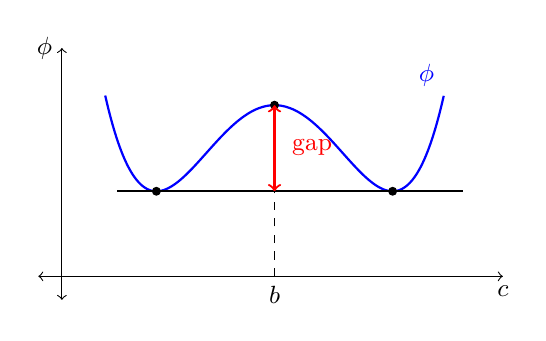
\begin{tikzpicture}[scale=1.0]
    \draw[<->] (-0.3,0) -- (5.6,0) node[anchor=north] {\small $c$};
    \draw[<->] (0,-0.3) -- (0,2.9) node[anchor=east] {\small $\phi$};
    % phi(c) = 1.8*(0.12 (c-1.2)^2 (c-4.2)^2 + 0.6): two minima at c=1.2, 4.2 of height 1.08
    \draw[thick, samples=140, smooth, domain=0.55:4.85, color=blue]
        plot (\x, {1.8*(0.12*(\x-1.2)*(\x-1.2)*(\x-4.2)*(\x-4.2) + 0.6)});
    \draw[thick] (0.7,1.08) -- (5.1,1.08);
    \filldraw (2.7,2.1735) circle (1.4pt);
    \filldraw (1.2,1.08) circle (1.4pt);
    \filldraw (4.2,1.08) circle (1.4pt);
    \draw[<->, thick, color=red] (2.7,2.1735) -- (2.7,1.08);
    \node[anchor=west, color=red] at (2.8,1.63) {\small gap};
    \draw[dashed] (2.7,0) -- (2.7,1.08);
    \node[anchor=north] at (2.7,0) {\small $b$};
    \node[anchor=south east, color=blue] at (4.85,2.29) {\small $\phi$};
\end{tikzpicture}
\end{center}

\subsection{Shadow Prices}

We finish this section with the interpretation of Lagrange multipliers that gives them their name in economics, and which explains the strange sign conventions.

Imagine a factory that makes $n$ products out of $m$ raw materials. If it makes quantities $x = (x_1, \dots, x_n)$ then it makes profit $f(x)$ (we will minimize $-f$, but let us think in terms of maximizing profit), and producing $x$ consumes $h_j(x)$ units of raw material $j$. The factory has $b_j$ units of material $j$ available. So the factory owner solves `maximize $f(x)$ subject to $h(x) \leq b$'.

Now a supplier turns up and offers a small extra quantity $\varepsilon = (\varepsilon_1, \dots, \varepsilon_m)$ of raw materials. How much should the owner be willing to pay? The new optimal profit is $\phi(b + \varepsilon)$, so the increase is
$$
\phi(b + \varepsilon) - \phi(b) \approx \sum_{j = 1}^m\frac{\partial\phi}{\partial b_j}(b)\,\varepsilon_j.
$$
The quantity $\partial\phi/\partial b_j$ is the marginal value to this factory of one more unit of material $j$: it is called the \vocab{shadow price} of material $j$. It is a `shadow' price because it is invisible from outside -- it depends entirely on the internal state of the factory, not on the market.

\begin{theorem}
    If $\phi$ is differentiable at $b$ and has a supporting hyperplane at $b$ with normal $\lambda$, then $\lambda = \nabla\phi(b)$.
\end{theorem}
\begin{proof}
    Let $a \in \R^m$ be arbitrary and $\delta > 0$. The supporting hyperplane condition at $c = b + \delta a$ gives
    $$
    \phi(b + \delta a) - \phi(b) \geq \delta\, \lambda\cdot a, \quad\text{ so }\quad \frac{\phi(b + \delta a) - \phi(b)}{\delta} \geq \lambda\cdot a.
    $$
    Letting $\delta \rightarrow 0$ and using differentiability, $\nabla\phi(b)\cdot a \geq \lambda\cdot a$. Since $a$ was arbitrary we may also apply this with $-a$, giving $\nabla\phi(b)\cdot a = \lambda\cdot a$ for all $a$, and hence $\lambda = \nabla\phi(b)$.
\end{proof}

\begin{example}
    Let us verify this in a case where we can compute everything. Consider
    $$
    \text{minimize } \tfrac12(x_1^2 + x_2^2) \text{ subject to } x_1 + x_2 = b,
    $$
    over $x \in \R^2$. The Lagrangian is
    $$
    L(x,\lambda) = \tfrac12(x_1^2 + x_2^2) - \lambda(x_1 + x_2 - b) = \left(\tfrac12x_1^2 - \lambda x_1\right) + \left(\tfrac12 x_2^2 - \lambda x_2\right) + \lambda b,
    $$
    which is bounded below for every $\lambda$, so $\Lambda = \R$. Minimizing each bracket gives $x_1 = x_2 = \lambda$, and feasibility then forces $2\lambda = b$, so
    $$
    \lambda^* = \frac b2, \qquad x^* = \left(\frac b2, \frac b2\right), \qquad \phi(b) = \frac{b^2}{4}.
    $$
    And indeed $\phi'(b) = b/2 = \lambda^*$, exactly as the theorem promises. Concretely: relaxing the constraint from $b$ to $b + \varepsilon$ increases the optimal cost by about $\lambda^*\varepsilon$.
\end{example}

So the Lagrange multipliers \emph{are} the shadow prices. This makes complementary slackness completely intuitive: if a raw material is not fully used up ($s_j > 0$, the constraint is slack) then an extra unit of it is worth nothing, so its shadow price $\lambda_j$ is zero. Conversely, if it has a nonzero price then we must be using every last unit of it.

There is a matching interpretation of the dual problem. Think of it from the supplier's point of view. The supplier posts prices $\lambda$ for the raw materials and offers to buy the finished products. Given prices $\lambda$, the factory owner will choose $x$ to maximize
$$
\underbrace{f(x)}_{\text{revenue}} - \underbrace{\lambda\cdot(h(x) - b)}_{\text{cost of materials}},
$$
which is exactly the Lagrangian. The supplier, knowing this, chooses $\lambda$ to make the factory owner's best achievable profit as small as possible -- that is, the supplier solves the dual problem. Weak duality says the supplier can never squeeze the owner below the true optimum, and strong duality says that with the right prices the two coincide: at equilibrium there is no advantage to either party.

\section{Linear Programming}

We now specialize to the case where everything in sight is linear. This may sound like a drastic restriction, and in a sense it is, but linear programs are astonishingly expressive -- an enormous fraction of the optimization problems that actually arise in industry are linear programs, or are usefully approximated by them. More importantly for us, in this setting the general theory of the previous section becomes completely explicit and computable, and we will be able to write down an algorithm that solves any linear program by hand.

\subsection{Linear Programs}

\begin{definition}[Linear Program]
    A \vocab{linear program} is an optimization problem in which the objective function and all of the constraints are linear (more precisely, affine) functions of the decision variables.
\end{definition}

A general linear program might look something like
\begin{alignat*}{2}
    & \text{minimize} \quad && 2x_1 - x_2 + 4x_3 \\
    & \text{subject to} \quad && x_1 + x_2 + x_4 \leq 2, \\
    & && 3x_2 - x_3 = 5,\\
    & && x_3 + x_4 \geq 3,\\
    & && x_1 \geq 0,\ x_3 \leq 0,
\end{alignat*}
with $x_2$ and $x_4$ unconstrained in sign. This is a mess of different constraint types, and before doing anything we would like to tidy it up. Happily, all of the constraint types are interchangeable.

\begin{definition}[Equivalent Problems]
    Two optimization problems are \vocab{equivalent} if from a feasible solution to either one we can construct a feasible solution to the other with the same cost. Rewriting a problem as an equivalent one is called \vocab{reduction}.
\end{definition}

The reductions we need are all elementary:
\begin{itemize}
    \item $a\cdot x \leq b$ becomes $-a\cdot x \geq -b$;
    \item $a \cdot x \geq b$ becomes $a\cdot x - s = b$ with $s \geq 0$ (a \emph{surplus} variable), and $a\cdot x \leq b$ becomes $a\cdot x + s = b$ with $s \geq 0$ (a \emph{slack} variable);
    \item $a\cdot x = b$ becomes the pair $a\cdot x \geq b$ and $-a\cdot x \geq -b$;
    \item a variable $x_j \leq 0$ is replaced by $-x_j \geq 0$;
    \item a variable $x_j$ of unrestricted sign is replaced by $x_j^+ - x_j^-$ with $x_j^+, x_j^- \geq 0$.
\end{itemize}
Applying these as needed, we can put any linear program into either of two standard shapes.

\begin{definition}[General and Standard Form]
    A linear program is in \vocab{general form} if it is written
    \begin{alignat*}{2}
        & \text{minimize} \quad && c \cdot x \\
        & \text{subject to} \quad && Ax \geq b,
    \end{alignat*}
    and in \vocab{standard form} if it is written
    \begin{alignat*}{2}
        & \text{minimize} \quad && c \cdot x \\
        & \text{subject to} \quad && Ax = b, \\
        & && x \geq 0,
    \end{alignat*}
    where in both cases $A \in \R^{m\times n}$, $b \in \R^m$ and $c \in \R^n$.
\end{definition}

Standard form is what we will use for computation, since the constraint $Ax = b$ is just a linear system; general form is convenient for stating duality. Both are fully general: to get from general to standard form, first introduce surplus variables to turn $Ax \geq b$ into $Ax - s = b$ with $s \geq 0$, then split each unrestricted $x_j$ as $x_j^+ - x_j^-$, giving
\begin{alignat*}{2}
    & \text{minimize} \quad && c\cdot x^+ - c\cdot x^- \\
    & \text{subject to} \quad && Ax^+ - Ax^- - s = b, \\
    & && x^+, x^-, s \geq 0,
\end{alignat*}
which is in standard form in the variables $(x^+, x^-, s) \in \R^{2n + m}_{\geq 0}$.

Notice that reduction to standard form typically increases the number of variables. That is fine: what matters is that the constraint matrix stays sparse and the structure stays linear.

\subsection{A Two-Dimensional Example}

Before doing any theory, it is worth solving a small linear program by drawing a picture, because the picture explains everything that follows.

\begin{example}
    Consider the problem
    \begin{alignat*}{2}
        & \text{maximize} \quad && x_1 + x_2 \\
        & \text{subject to} \quad && x_1 + 2x_2 \leq 6, \\
        & && x_1 - x_2 \leq 3,\\
        & && x_1, x_2 \geq 0.
    \end{alignat*}
    The feasible set is the shaded polygon below: the intersection of four half-planes. The dashed lines are the level sets $x_1 + x_2 = \text{const}$ of the objective, which all have gradient $(1,1)$. To maximize the objective, we slide the dashed line in the direction $(1,1)$ as far as we can while still touching the feasible set.
\end{example}

\begin{center}
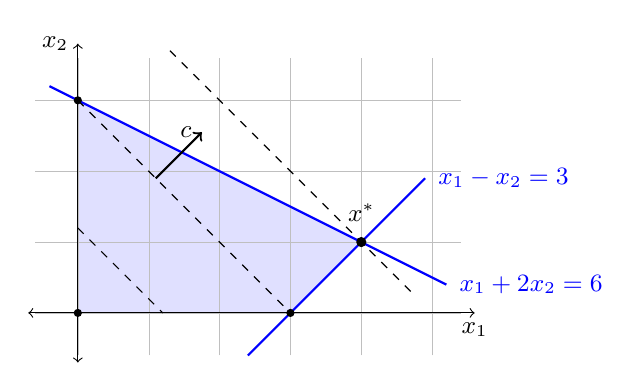
\begin{tikzpicture}[scale=0.9]
    \fill[color=blue!12] (0,0) -- (3,0) -- (4,1) -- (0,3) -- cycle;
    \draw[ultra thin, color=lightgray] (-0.6,-0.6) grid (5.4,3.6);
    \draw[<->] (-0.7,0) -- (5.6,0) node[anchor=north] {\small $x_1$};
    \draw[<->] (0,-0.7) -- (0,3.8) node[anchor=east] {\small $x_2$};
    % x1 + 2x2 = 6
    \draw[thick, color=blue] (-0.4,3.2) -- (5.2,0.4);
    \node[anchor=west, color=blue] at (5.25,0.4) {\small $x_1 + 2x_2 = 6$};
    % x1 - x2 = 3
    \draw[thick, color=blue] (2.4,-0.6) -- (4.9,1.9);
    \node[anchor=west, color=blue] at (4.95,1.9) {\small $x_1 - x_2 = 3$};
    % objective contours: x1 + x2 = k
    \draw[dashed] (0,1.2) -- (1.2,0);
    \draw[dashed] (0,3.0) -- (3.0,0);
    \draw[dashed] (1.3,3.7) -- (4.7,0.3);
    \draw[->, thick] (1.1,1.9) -- (1.75,2.55) node[anchor=east] {\small $c$};
    \filldraw (4,1) circle (1.8pt);
    \node[anchor=south] at (4,1.15) {\small $x^*$};
    \filldraw (3,0) circle (1.4pt);
    \filldraw (0,3) circle (1.4pt);
    \filldraw (0,0) circle (1.4pt);
\end{tikzpicture}
\end{center}

The optimum is at $x^* = (4,1)$, where the two constraint lines meet, with optimal value $5$. Two features of this picture are completely general, and are the theoretical backbone of linear programming:
\begin{enumerate}[label=(\roman*)]
    \item the feasible set is a \emph{polyhedron} -- an intersection of finitely many half-spaces; and
    \item the optimum is attained at a \emph{corner} of that polyhedron.
\end{enumerate}
If the objective happens to be parallel to one of the edges, then a whole edge is optimal -- but even then, a corner is among the optimal points. So to solve a linear program, it suffices to search the (finitely many!) corners. Our next job is to say precisely what a corner is, algebraically.

\subsection{Extreme Points}

\begin{definition}[Extreme Point]
    A point $x$ in a convex set $C$ is an \vocab{extreme point} if it cannot be written as $x = \delta y + (1 - \delta)z$ for $y, z \in C$ with $y \neq z$ and $\delta \in (0,1)$. That is, $x$ does not lie strictly inside any line segment contained in $C$.
\end{definition}

\begin{center}
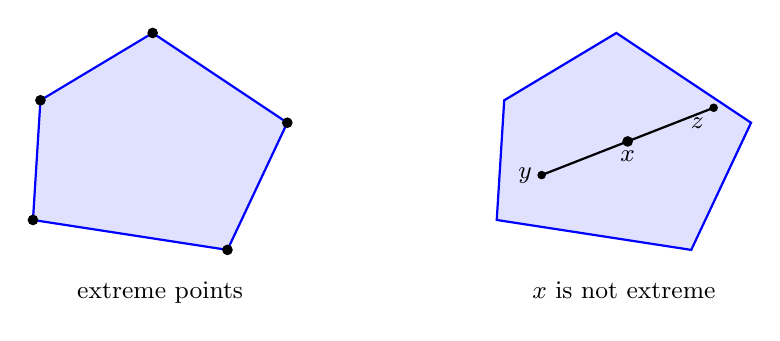
\begin{tikzpicture}[scale=0.95]
    \fill[color=blue!12] (0,0) -- (2.6,-0.4) -- (3.4,1.3) -- (1.6,2.5) -- (0.1,1.6) -- cycle;
    \draw[thick, color=blue] (0,0) -- (2.6,-0.4) -- (3.4,1.3) -- (1.6,2.5) -- (0.1,1.6) -- cycle;
    \filldraw (0,0) circle (1.8pt);
    \filldraw (2.6,-0.4) circle (1.8pt);
    \filldraw (3.4,1.3) circle (1.8pt);
    \filldraw (1.6,2.5) circle (1.8pt);
    \filldraw (0.1,1.6) circle (1.8pt);
    \node[anchor=north] at (1.7,-0.7) {\small extreme points};
    \begin{scope}[xshift=6.2cm]
    \fill[color=blue!12] (0,0) -- (2.6,-0.4) -- (3.4,1.3) -- (1.6,2.5) -- (0.1,1.6) -- cycle;
    \draw[thick, color=blue] (0,0) -- (2.6,-0.4) -- (3.4,1.3) -- (1.6,2.5) -- (0.1,1.6) -- cycle;
    \draw[thick] (0.6,0.6) -- (2.9,1.5);
    \filldraw (0.6,0.6) circle (1.4pt) node[anchor=east] {\small $y$};
    \filldraw (2.9,1.5) circle (1.4pt) node[anchor=north east] {\small $z$};
    \filldraw (1.75,1.05) circle (1.8pt) node[anchor=north] {\small $x$};
    \node[anchor=north] at (1.7,-0.7) {\small $x$ is not extreme};
    \end{scope}
\end{tikzpicture}
\end{center}

The relevance is the following general fact, which explains observation (ii) above.

\begin{proposition}
    Let $f$ be a convex function on a convex set $C$, and let $y, z \in C$. Then $f$ attains its maximum over the segment $[y,z]$ at an endpoint. Consequently, if $C$ is a bounded polyhedron then $\max_{x \in C}f(x)$ is attained at an extreme point of $C$.
\end{proposition}
\begin{proof}
    For the first part, if $x = \delta y + (1-\delta)z$ then by convexity
    $$
    f(x) \leq \delta f(y) + (1 - \delta)f(z) \leq \max\{f(y), f(z)\}.
    $$
    For the second, every point of a bounded polyhedron $C$ can be written as a convex combination $x = \sum_{i=1}^k \delta_i x^{(i)}$ of extreme points $x^{(i)}$, with $\delta_i \geq 0$ and $\sum\delta_i = 1$. By convexity again,
    $$
    f(x) \leq \sum_{i = 1}^k \delta_i f(x^{(i)}) \leq \max_i f(x^{(i)}),
    $$
    so no interior point beats the best extreme point.
\end{proof}

Since a linear function is convex (and concave), the maximum \emph{and} the minimum of a linear function on a bounded polyhedron are both attained at extreme points. So the corners really are all we need to look at. What we lack is a way of finding them without drawing a picture, which is hopeless in $\R^{100}$.

\subsection{Basic Solutions}

Consider now a linear program in standard form,
\begin{alignat*}{2}
    & \text{minimize} \quad && c \cdot x \\
    & \text{subject to} \quad && Ax = b, \\
    & && x \geq 0,
\end{alignat*}
with $A \in \R^{m \times n}$ and typically $n > m$, so that $Ax = b$ is an underdetermined system with a whole affine space of solutions. Intuitively, a corner of the feasible set is a point where as many constraints as possible are tight; since the only inequality constraints are $x_j \geq 0$, this means a point with as many zero coordinates as possible.

\begin{definition}[Basic Solution]
    A vector $x \in \R^n$ is a \vocab{basic solution} of $Ax = b$ if $Ax = b$ and $x$ has at most $m$ nonzero entries. If in addition $x \geq 0$, it is a \vocab{basic feasible solution} (bfs).
\end{definition}

To construct basic solutions, we choose which $m$ coordinates are allowed to be nonzero. We make two standing assumptions on $A$, both harmless.
\begin{enumerate}[label=(\Alph*)]
    \item The $m$ rows of $A$ are linearly independent. (Otherwise some constraint is redundant or inconsistent, and we can delete it.)
    \item Every set of $m$ columns of $A$ is linearly independent. (This is a genericity assumption; we can always perturb $b$ slightly to arrange it.)
\end{enumerate}

Given a choice of indices $B = \{B(1), \dots, B(m)\} \subseteq \{1, \dots, n\}$, write $A_j$ for the $j$th column of $A$ and let
$$
A_B = \begin{pmatrix} A_{B(1)} & \cdots & A_{B(m)}\end{pmatrix} \in \R^{m\times m}
$$
be the corresponding \vocab{basis matrix}. Setting $x_j = 0$ for $j \notin B$, the equation $Ax = b$ reduces to $A_B x_B = b$, where $x_B = (x_{B(1)}, \dots, x_{B(m)})$. By assumption (B), $A_B$ is invertible, and so
$$
x_B = A_B^{-1}b.
$$
The indices in $B$ are the \vocab{basic indices}, the corresponding variables are the \vocab{basic variables}, and the rest are the \vocab{non-basic variables} (all set to zero). If moreover $A_B^{-1}b \geq 0$, we have found a basic feasible solution.

\begin{enumerate}[label=(\Alph*)]
    \setcounter{enumi}{2}
    \item (\vocab{Non-degeneracy}) Every basic solution has \emph{exactly} $m$ nonzero entries.
\end{enumerate}
This last assumption is not without loss of generality, and we will discuss what goes wrong without it in Section \ref{sec:degeneracy}. Until then we assume it.

Now we can connect the algebra to the geometry.

\begin{theorem}[Basic Feasible Solutions are Extreme Points]
    Let $P = \{x : Ax = b, x \geq 0\}$. Then $x$ is an extreme point of $P$ if and only if $x$ is a basic feasible solution.
\end{theorem}
\begin{proof}
    Suppose first that $x$ is a bfs, with basis $B$, and suppose $x = \delta y + (1 - \delta)z$ with $y, z \in P$ and $\delta \in (0,1)$. For $j \notin B$ we have $x_j = 0$, so $\delta y_j + (1-\delta)z_j = 0$; but $y_j, z_j \geq 0$ and $\delta \in (0,1)$, so $y_j = z_j = 0$. Hence $y$ and $z$ are also supported on $B$, and $A_B y_B = b = A_B z_B$. As $A_B$ is invertible, $y_B = z_B = A_B^{-1}b = x_B$, and so $y = z = x$. Thus $x$ is extreme.

    Conversely suppose $x \in P$ is not a bfs, so $x$ has $r > m$ nonzero entries, say in positions $i_1, \dots, i_r$. The columns $A_{i_1}, \dots, A_{i_r}$ are $r > m$ vectors in $\R^m$, hence linearly dependent: there are weights $w_{i_1}, \dots, w_{i_r}$, not all zero, with
    $$
    w_{i_1}A_{i_1} + \cdots + w_{i_r}A_{i_r} = 0.
    $$
    Extend $w$ to a vector in $\R^n$ by setting $w_i = 0$ for $i \notin \{i_1, \dots, i_r\}$. Then $w \neq 0$ and $Aw = 0$, so $A(x \pm \varepsilon w) = b$ for every $\varepsilon$. Moreover $w$ is supported where $x$ is strictly positive, so for small enough $\varepsilon > 0$ we have $x \pm \varepsilon w \geq 0$, i.e.\ $x \pm \varepsilon w \in P$. But then $x$ is the midpoint of these two distinct points of $P$, so $x$ is not extreme.
\end{proof}

\begin{corollary}
    There are at most $\binom{n}{m}$ basic solutions, and hence at most $\binom{n}{m}$ extreme points of $P$.
\end{corollary}

\begin{example}
    Let us see this explicitly on the example of Section 3.2. Writing it as a minimization and adding slack variables $x_3, x_4$, the standard form is: minimize $-x_1 - x_2$ subject to
    $$
    x_1 + 2x_2 + x_3 = 6, \qquad x_1 - x_2 + x_4 = 3, \qquad x \geq 0,
    $$
    so $m = 2$, $n = 4$ and there are at most $\binom42 = 6$ basic solutions. Let us list them all.
    \begin{center}
    \begin{tabular}{c|c|c|c}
        basis & $x = (x_1,x_2,x_3,x_4)$ & feasible? & cost \\\hline
        $\{3,4\}$ & $(0,0,6,3)$ & yes & $0$ \\
        $\{1,3\}$ & $(3,0,3,0)$ & yes & $-3$ \\
        $\{1,4\}$ & $(6,0,0,-3)$ & no & --- \\
        $\{2,3\}$ & $(0,-3,12,0)$ & no & --- \\
        $\{2,4\}$ & $(0,3,0,6)$ & yes & $-3$ \\
        $\{1,2\}$ & $(4,1,0,0)$ & yes & $-5$
    \end{tabular}
    \end{center}
    For instance, for the basis $\{1,2\}$ we set $x_3 = x_4 = 0$ and solve $x_1 + 2x_2 = 6$, $x_1 - x_2 = 3$, giving $(x_1, x_2) = (4,1)$. Comparing with the picture in Section 3.2, the four basic feasible solutions are exactly the four corners $(0,0)$, $(3,0)$, $(0,3)$ and $(4,1)$ of the polygon, and the two infeasible basic solutions are the points $(6,0)$ and $(0,-3)$ where two constraint lines meet \emph{outside} the feasible region. The best cost among the feasible ones is $-5$ at $(4,1)$, in agreement with what we found geometrically.
\end{example}

\begin{theorem}[Fundamental Theorem of Linear Programming]
    If a linear program in standard form is feasible and bounded, then there is an optimal solution which is a basic feasible solution.
\end{theorem}
\begin{proof}
    Let $x$ be an optimal solution with as few nonzero entries as possible, say $r$ of them. If $r \leq m$ then $x$ is a bfs and we are done, so suppose $r > m$. By the argument in the previous proof, there is $w \neq 0$ with $Aw = 0$, supported on the positions where $x$ is nonzero.

    Consider $x_\theta = x + \theta w$, which satisfies $Ax_\theta = b$ for all $\theta \in \R$, and lies in $P$ for all $\theta$ in some interval around $0$. Its cost is $c\cdot x + \theta (c\cdot w)$. If $c\cdot w \neq 0$ then choosing the sign of $\theta$ appropriately strictly decreases the cost, contradicting optimality of $x$. So $c\cdot w = 0$ and $x_\theta$ is optimal for every feasible $\theta$.

    Now increase $|\theta|$ (in either direction) until some coordinate of $x_\theta$ first hits zero -- this happens for a finite $\theta$ since $w$ is nonzero and supported where $x$ is. The resulting point is optimal, feasible, and has strictly fewer than $r$ nonzero entries, contradicting minimality of $r$.
\end{proof}

This is genuinely good news: it reduces an optimization over a continuum to a search over a finite set. The bad news is that $\binom{n}{m}$ is astronomically large -- for $n = 100$ and $m = 50$ it exceeds $10^{29}$ -- so brute force is out of the question. The simplex method, which we come to shortly, is a clever way of walking from one basic feasible solution to a better one.

\subsection{Duality for Linear Programs}

Before the algorithm, let us work out what the duality theory of Section 2 says here. It says something extremely concrete.

Consider a linear program in general form, with surplus variables added:
\begin{alignat*}{2}
    & \text{minimize} \quad && c\cdot x \\
    & \text{subject to} \quad && Ax - s = b, \\
    & && s \geq 0,
\end{alignat*}
where $x$ is unrestricted. The Lagrangian is
$$
L(x, s, \lambda) = c\cdot x - \lambda\cdot(Ax - s - b) = (c - A^T\lambda)\cdot x + \lambda\cdot s + \lambda\cdot b.
$$
Since $x$ ranges over all of $\R^n$, this is bounded below only if $c - A^T\lambda = 0$; and since $s$ ranges over $[0,\infty)^m$, we need $\lambda \geq 0$. Given both, the infimum is attained at $s = 0$ and equals $\lambda\cdot b$. Hence
$$
\Lambda = \{\lambda : A^T\lambda = c,\ \lambda \geq 0\}, \qquad g(\lambda) = \lambda\cdot b,
$$
and we have proved the following.

\begin{proposition}[Dual of a General-Form LP]
    The dual of
    \begin{alignat*}{2}
        & \text{minimize} \quad && c\cdot x \quad\text{ subject to } \quad Ax \geq b
    \end{alignat*}
    is
    \begin{alignat*}{2}
        & \text{maximize} \quad && \lambda \cdot b \quad\text{ subject to }\quad A^T\lambda = c,\ \lambda \geq 0.
    \end{alignat*}
\end{proposition}

Notice that the dual of a general-form problem is in standard form. The same computation for a standard-form primal gives the reverse.

\begin{proposition}[Dual of a Standard-Form LP]
    The dual of
    \begin{alignat*}{2}
        & \text{minimize} \quad && c\cdot x \quad\text{ subject to } \quad Ax = b,\ x \geq 0
    \end{alignat*}
    is
    \begin{alignat*}{2}
        & \text{maximize} \quad && \lambda \cdot b \quad\text{ subject to }\quad A^T\lambda \leq c.
    \end{alignat*}
\end{proposition}
\begin{proof}
    Here $X = \{x : x \geq 0\}$ and $L(x,\lambda) = c\cdot x - \lambda\cdot(Ax - b) = (c - A^T\lambda)\cdot x + \lambda\cdot b$. Since $x$ ranges over the non-negative orthant, this is bounded below exactly when $c - A^T\lambda \geq 0$, and then the infimum is attained at $x = 0$ and equals $\lambda\cdot b$.
\end{proof}

These two facts fit together neatly.

\begin{proposition}
    The dual of the dual is the primal.
\end{proposition}
\begin{proof}
    Start with the standard-form primal and its dual `maximize $\lambda\cdot b$ subject to $A^T\lambda \leq c$'. Rewrite this as a minimization in general form: putting $\mu = -\lambda$,
    $$
    \text{minimize } \mu\cdot b \text{ subject to } A^T\mu \geq -c,
    $$
    whose optimal value is the negative of the original. Applying the general-form dual with data $(b, A^T, -c)$ in place of $(c, A, b)$, the dual is
    $$
    \text{maximize } -\theta\cdot c \text{ subject to } A\theta = b,\ \theta \geq 0,
    $$
    that is, minimize $c\cdot\theta$ subject to $A\theta = b$, $\theta \geq 0$, which is the original primal.
\end{proof}

For a completely general linear program, the pattern of the dual is worth recording; each of these can be derived by the reductions above.

\begin{proposition}[Dual of a General Linear Program]
    The dual of
    \begin{alignat*}{3}
        & \text{minimize} \quad && c\cdot x && \\
        & \text{subject to} \quad && a_i \cdot x \geq b_i \quad&& i \in M_1,\\
        & && a_i \cdot x \leq b_i && i \in M_2,\\
        & && a_i \cdot x = b_i && i \in M_3,\\
        & && x_j \geq 0 && j \in N_1,\\
        & && x_j \leq 0 && j \in N_2,\\
        & && x_j \text{ free} && j \in N_3,
    \end{alignat*}
    is
    \begin{alignat*}{3}
        & \text{maximize} \quad && \lambda \cdot b && \\
        & \text{subject to} \quad && \lambda_i \geq 0 \quad&& i \in M_1,\\
        & && \lambda_i \leq 0 && i \in M_2,\\
        & && \lambda_i \text{ free} && i \in M_3,\\
        & && \lambda\cdot A_j \leq c_j && j \in N_1,\\
        & && \lambda \cdot A_j \geq c_j && j \in N_2,\\
        & && \lambda\cdot A_j = c_j && j \in N_3.
    \end{alignat*}
\end{proposition}

The mnemonic is that constraints in the primal correspond to variables in the dual and vice versa. It is worth having the correspondence in a table:
\begin{center}
\begin{tabular}{l|l}
    primal (minimize) & dual (maximize)\\\hline
    $i$th constraint $\geq$ & $i$th variable $\geq 0$\\
    $i$th constraint $\leq$ & $i$th variable $\leq 0$\\
    $i$th constraint $=$ & $i$th variable free\\\hline
    $j$th variable $\geq 0$ & $j$th constraint $\leq$\\
    $j$th variable $\leq 0$ & $j$th constraint $\geq$\\
    $j$th variable free & $j$th constraint $=$\\\hline
    objective vector $c$ & right-hand side $c$\\
    right-hand side $b$ & objective vector $b$\\
    constraint matrix $A$ & constraint matrix $A^T$
\end{tabular}
\end{center}
There is an easy way to remember the direction of the inequalities: whichever choice makes weak duality come out right is the correct one. For instance in the standard-form case, a primal variable $x_j \geq 0$ contributes $c_jx_j$ to the objective, and we need $(c_j - \lambda\cdot A_j)x_j \geq 0$ for the bound $c\cdot x \geq \lambda\cdot b$ to work; with $x_j \geq 0$ this forces $\lambda\cdot A_j \leq c_j$, which is a $\leq$ constraint in the dual.

Since a linear program has a convex objective, convex constraints and convex feasible region, the theorem of Section 2.4 applies immediately.

\begin{theorem}[Strong Duality for Linear Programs]
    If a linear program is feasible and bounded, then so is its dual, and their optimal values are equal.
\end{theorem}
\begin{proof}
    The value function $\phi(d) = \inf\{c\cdot x : Ax \geq d\}$ is convex by the theorem in Section 2.4 (taking $X = \R^n$, and noting that $f(x) = c\cdot x$ and $h(x) = -Ax$ are linear, hence convex). Hence $\phi$ has a supporting hyperplane at $b$, and strong duality holds.
\end{proof}

\subsection{Complementary Slackness for Linear Programs}

Strong duality gives us a certificate of optimality, and in the linear case that certificate takes an extremely usable form.

\begin{theorem}[Optimality Conditions]
    Let $x$ be feasible for the primal and $\lambda$ feasible for the dual, in the general setting of the previous proposition. Then $x$ and $\lambda$ are both optimal if and only if
    \begin{enumerate}[label=(\roman*)]
        \item $\lambda_i(a_i\cdot x - b_i) = 0$ for all $i$, and
        \item $(c_j - \lambda\cdot A_j)x_j = 0$ for all $j$.
    \end{enumerate}
\end{theorem}
\begin{proof}
    Set $u_i = \lambda_i(a_i\cdot x - b_i)$ and $v_j = (c_j - \lambda\cdot A_j)x_j$. Feasibility of $x$ and $\lambda$ makes each $u_i \geq 0$ and each $v_j \geq 0$: for instance if $i \in M_1$ then $a_i\cdot x - b_i \geq 0$ and $\lambda_i \geq 0$, while if $i \in M_2$ both factors flip sign, and if $i \in M_3$ the second factor is zero. The same case analysis works for $v_j$. Now
    $$
    \sum_i u_i = \lambda\cdot(Ax) - \lambda\cdot b, \qquad \sum_j v_j = c\cdot x - \lambda \cdot (Ax),
    $$
    so adding,
    $$
    0 \leq \sum_i u_i + \sum_j v_j = c\cdot x - \lambda\cdot b.
    $$
    If (i) and (ii) hold then all $u_i, v_j$ vanish, so $c\cdot x = \lambda\cdot b$, and by weak duality both must be optimal. Conversely if both are optimal then strong duality gives $c\cdot x = \lambda\cdot b$, so $\sum u_i + \sum v_j = 0$; as all the terms are non-negative, they must all be zero.
\end{proof}

Conditions (i) and (ii) are the \vocab{complementary slackness} conditions for a linear program. Condition (i) says: if the dual variable $\lambda_i$ is nonzero then the $i$th primal constraint is tight. Condition (ii) says: if the primal variable $x_j$ is nonzero then the $j$th dual constraint is tight. So the whole state of the optimum is captured by:
\begin{center}
    primal feasibility \quad + \quad dual feasibility \quad + \quad complementary slackness.
\end{center}
These three conditions are what the simplex method will maintain and enforce, and the algorithm can be understood entirely in terms of them: it keeps the first and third true at all times, and works to make the second true.

\begin{example}
    Return to our two-dimensional example, written as a minimization in general form. We minimize $-x_1 - x_2$ subject to
    $$
    \begin{pmatrix} -1 & -2 \\ -1 & 1 \\ 1 & 0 \\ 0 & 1\end{pmatrix}\begin{pmatrix}x_1\\x_2\end{pmatrix} \geq \begin{pmatrix}-6\\-3\\0\\0\end{pmatrix}.
    $$
    The dual is: maximize $-6\lambda_1 - 3\lambda_2$ subject to $\lambda \geq 0$ and
    $$
    -\lambda_1 - \lambda_2 + \lambda_3 = -1, \qquad -2\lambda_1 + \lambda_2 + \lambda_4 = -1.
    $$
    At the primal optimum $x^* = (4,1)$ the first two constraints are tight and the last two are slack, so complementary slackness forces $\lambda_3 = \lambda_4 = 0$. The remaining equations give $\lambda_1 + \lambda_2 = 1$ and $2\lambda_1 - \lambda_2 = 1$, so $\lambda = (2/3, 1/3, 0, 0)$, which is indeed non-negative. The dual objective is $-6\cdot\frac23 - 3\cdot\frac13 = -5$, matching the primal optimal value of $-5$. So each certifies the other.

    The shadow price interpretation is now concrete: $\lambda_1 = 2/3$ says that relaxing the first constraint from $x_1 + 2x_2 \leq 6$ to $\leq 7$ would increase the maximum of $x_1 + x_2$ by $2/3$.
\end{example}

\section{The Simplex Method}

We know that an optimal solution can be found among the basic feasible solutions, and we know that there are far too many of these to enumerate. The \vocab{simplex method}, due to Dantzig, resolves this by moving from one basic feasible solution to an adjacent one, always decreasing the cost, until no improving move exists. Geometrically, it walks along the edges of the feasible polyhedron from corner to corner, downhill all the way.

\begin{center}
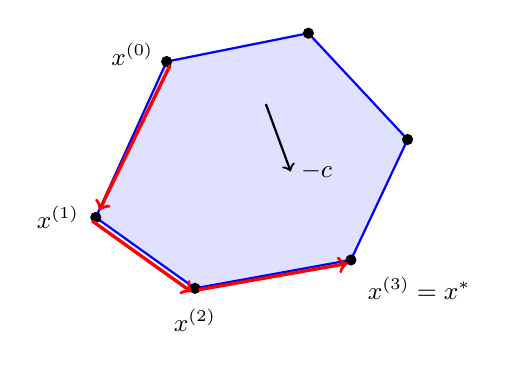
\begin{tikzpicture}[scale=0.9]
    \fill[color=blue!12] (0,0.4) -- (1.4,-0.6) -- (3.6,-0.2) -- (4.4,1.5) -- (3.0,3.0) -- (1.0,2.6) -- cycle;
    \draw[thick, color=blue] (0,0.4) -- (1.4,-0.6) -- (3.6,-0.2) -- (4.4,1.5) -- (3.0,3.0) -- (1.0,2.6) -- cycle;
    \filldraw (1.0,2.6) circle (2.0pt);
    \filldraw (0,0.4) circle (2.0pt);
    \filldraw (1.4,-0.6) circle (2.0pt);
    \filldraw (3.6,-0.2) circle (2.0pt);
    \filldraw (4.4,1.5) circle (2.0pt);
    \filldraw (3.0,3.0) circle (2.0pt);
    \draw[->, very thick, color=red] (1.05,2.55) -- (0.05,0.5);
    \draw[->, very thick, color=red] (-0.05,0.35) -- (1.35,-0.65);
    \draw[->, very thick, color=red] (1.45,-0.62) -- (3.55,-0.25);
    \node[anchor=east] at (0.95,2.7) {\small $x^{(0)}$};
    \node[anchor=east] at (-0.1,0.4) {\small $x^{(1)}$};
    \node[anchor=north] at (1.4,-0.75) {\small $x^{(2)}$};
    \node[anchor=north west] at (3.7,-0.3) {\small $x^{(3)} = x^*$};
    \draw[->, thick] (2.4,2.0) -- (2.75,1.05) node[anchor=west] {\small $-c$};
\end{tikzpicture}
\end{center}

\subsection{Reduced Costs}

To turn the picture into an algorithm we need to answer two questions: when is a basic feasible solution optimal, and if it is not, which neighbouring solution should we move to? Both answers come from duality.

Suppose we are at a basic feasible solution $x$ with basis matrix $B = A_B$ (we will write $B$ for both the index set and the matrix, as is traditional). We have primal feasibility for free. Let us try to construct a $\lambda$ making complementary slackness hold, and then check whether it is dual feasible.

For a standard-form problem, the three optimality conditions read
\begin{itemize}
    \item (primal feasibility) $Ax = b$, $x \geq 0$;
    \item (dual feasibility) $A^T\lambda \leq c$;
    \item (complementary slackness) $x\cdot(c - A^T\lambda) = 0$.
\end{itemize}
Since $x_j = 0$ for non-basic $j$, complementary slackness only constrains the basic coordinates, where $x_B > 0$; so it forces $c_B - B^T\lambda = 0$, that is
$$
\lambda = (B^T)^{-1}c_B.
$$
With this choice of $\lambda$, primal feasibility and complementary slackness both hold. Only dual feasibility $A^T\lambda \leq c$ remains, and this motivates the following definition.

\begin{definition}[Reduced Costs]
    Given a basis $B$, the vector of \vocab{reduced costs} is
    $$
    \bar c = c - A^T(B^T)^{-1}c_B, \qquad\text{ componentwise }\qquad \bar c_j = c_j - c_B\cdot(B^{-1}A_j).
    $$
\end{definition}

By construction, dual feasibility is precisely the statement $\bar c \geq 0$, so we have proved most of the following.

\begin{theorem}[Optimality Criterion]
    Let $x$ be a basic feasible solution with basis $B$ and reduced cost vector $\bar c$. If $\bar c \geq 0$ then $x$ is optimal.
\end{theorem}

Note that $\bar c_j = 0$ for every basic $j$, since $B^{-1}A_{B(i)} = e_i$ and $c_B \cdot e_i = c_{B(i)}$. So we only need to inspect the non-basic reduced costs.

The reduced costs have a direct meaning too, which tells us what to do when some of them are negative. Suppose $j$ is non-basic and we try to increase $x_j$ from $0$ while keeping $Ax = b$. Formally, define the $j$th \vocab{basic direction} $d$ by $d_j = 1$, $d_i = 0$ for all other non-basic $i$, and $d_B$ determined by the requirement $Ad = 0$:
$$
Bd_B + A_j = 0 \implies d_B = -B^{-1}A_j.
$$
Then $A(x + \theta d) = b$ for all $\theta$, and since $x_B > 0$ (non-degeneracy!) we have $x + \theta d \geq 0$ for all small enough $\theta > 0$. So $d$ is a feasible direction. Its effect on the cost is
$$
c\cdot(x + \theta d) = c\cdot x + \theta\left(c_j - c_B\cdot(B^{-1}A_j)\right) = c\cdot x + \theta\,\bar c_j.
$$
So $\bar c_j$ is exactly the rate of change of the cost as we bring $x_j$ into the solution. If $\bar c_j < 0$, moving in the $j$th basic direction reduces the cost, and we should do so as far as possible.

How far can we go? We need $x + \theta d \geq 0$. The non-basic coordinates are fine ($x_j$ increases from $0$, the others stay at $0$). For the basic coordinates, writing $u = -d_B = B^{-1}A_j$, we need $x_{B(i)} - \theta u_i \geq 0$ for each $i$. If $u \leq 0$ this holds for all $\theta > 0$, and the cost is unbounded below. Otherwise the largest permissible step is
$$
\theta^* = \min_{\{i\, :\, u_i > 0\}}\frac{x_{B(i)}}{u_i},
$$
the so-called \vocab{ratio test}. Let $\ell$ attain the minimum. At $\theta = \theta^*$ the basic variable $x_{B(\ell)}$ becomes zero, so we have arrived at a new point with (again) $m$ nonzero entries: $x_j$ has entered the basis and $x_{B(\ell)}$ has left it.

\begin{theorem}
    With the notation above, $y = x + \theta^* d$ is a basic feasible solution with basis obtained from $B$ by replacing $A_{B(\ell)}$ with $A_j$, and $c\cdot y = c\cdot x + \theta^*\bar c_j < c\cdot x$.
\end{theorem}
\begin{proof}
    We have $Ay = b$ and $y \geq 0$ by the choice of $\theta^*$, and $y_{B(\ell)} = 0$ while $y_j = \theta^* > 0$, so exactly $m$ entries are nonzero and they sit in the claimed positions. The cost formula was computed above, and $\theta^* > 0$, $\bar c_j < 0$ give the strict decrease.
\end{proof}

Putting this together gives the algorithm.

\begin{definition}[The Simplex Method]
    To minimize $c\cdot x$ subject to $Ax = b$, $x \geq 0$:
    \begin{enumerate}[label=(\arabic*)]
        \item Start at a basic feasible solution $x$ with basis $B$.
        \item Compute the reduced costs $\bar c$. If $\bar c \geq 0$, stop: $x$ is optimal.
        \item Otherwise choose $j$ with $\bar c_j < 0$, and set $u = B^{-1}A_j$.
        \item If $u \leq 0$, stop: the problem is unbounded.
        \item Otherwise compute $\theta^* = \min\{x_{B(i)}/u_i : u_i > 0\}$, attained at $i = \ell$.
        \item Replace $B(\ell)$ by $j$ in the basis, update $x \mapsto x + \theta^* d$, and go to (2).
    \end{enumerate}
\end{definition}

Since the cost strictly decreases at each step (under the non-degeneracy assumption) we never revisit a basis, and there are finitely many bases, so the algorithm terminates.

\subsection{The Simplex Tableau}

Executing the algorithm as stated would require inverting $B$ at every step, which is intolerable by hand. The \vocab{tableau} is a bookkeeping device that maintains all of the required quantities automatically using row operations.

\begin{definition}[Simplex Tableau]
    The \vocab{simplex tableau} for the basis $B$ is the array
    $$
    \arraycolsep=6pt\def\arraystretch{1.4}
    \begin{array}{|c|c|}\hline
        -c_B\cdot x_B & \bar c^T \\\hline
        B^{-1}b & B^{-1}A \\\hline
    \end{array}
    $$
    or in more detail
    $$
    \arraycolsep=6pt\def\arraystretch{1.4}
    \begin{array}{|c|cccc|}\hline
        -c_B \cdot x_B & \bar c_1 & \bar c_2 & \cdots & \bar c_n \\\hline
        x_{B(1)} & \vdots & \vdots & & \vdots \\
        \vdots & B^{-1}A_1 & B^{-1}A_2 & \cdots & B^{-1}A_n\\
        x_{B(m)} & \vdots & \vdots & & \vdots\\\hline
    \end{array}
    $$
\end{definition}

So the top-left entry is minus the current cost, the top row holds the reduced costs, the left column holds the current basic feasible solution, and the body holds $B^{-1}A$ -- which is what the ratio test and basic directions need. Note that the basic columns of $B^{-1}A$ form an identity matrix, and the corresponding entries of the top row are zero; this is how we recognize the basis by looking at the tableau.

The remarkable fact -- and it really is worth pausing over -- is that the update in step (6) of the algorithm is achieved by pure Gaussian elimination on the tableau. The recipe is:
\begin{enumerate}[label=(\roman*)]
    \item Choose a \vocab{pivot column} $j$ with $\bar c_j < 0$.
    \item Choose the \vocab{pivot row} $\ell$ minimizing $x_{B(i)}/u_i$ among rows with $u_i > 0$, where $u_i$ is the entry in row $i$ of column $j$. The entry at $(\ell, j)$ is the \vocab{pivot}.
    \item Divide row $\ell$ by the pivot, then add multiples of row $\ell$ to every other row (including row $0$) so that column $j$ becomes the standard basis vector $e_\ell$.
\end{enumerate}
Why this works is not hard to see: multiplying on the left by $\bar B^{-1}B$ is exactly a sequence of row operations, and the row operations that turn column $j$ into $e_\ell$ are precisely those which implement the change of basis.

\begin{example}
    We solve
    \begin{alignat*}{2}
        & \text{minimize} \quad && -x_1 - x_2 - x_3 \\
        & \text{subject to} \quad && x_1 + 2x_2 + 2x_3 \leq 10, \\
        & && 2x_1 + x_2 + 2x_3 \leq 10, \\
        & && 2x_1 + 2x_2 + x_3 \leq 20, \\
        & && x_1, x_2, x_3 \geq 0.
    \end{alignat*}
    Adding slack variables $x_4, x_5, x_6 \geq 0$ puts this in standard form with
    $$
    A = \begin{pmatrix} 1&2&2&1&0&0\\2&1&2&0&1&0\\2&2&1&0&0&1\end{pmatrix}, \quad b = \begin{pmatrix}10\\10\\20\end{pmatrix}, \quad c = (-1,-1,-1,0,0,0).
    $$
    The slack variables give us a basic feasible solution for free: take $B = \{4,5,6\}$, so $B$ is the identity matrix and $x = (0,0,0,10,10,20)$. Since $c_B = 0$ we have $\bar c = c$ and cost $0$, and the initial tableau is
    $$
    \arraycolsep=6pt\def\arraystretch{1.3}
    \begin{array}{|c|cccccc|}\hline
        0 & -1 & -1 & -1 & 0 & 0 & 0\\\hline
        10 & 1 & 2 & 2 & 1 & 0 & 0\\
        10 & \boxed{2} & 1 & 2 & 0 & 1 & 0\\
        20 & 2 & 2 & 1 & 0 & 0 & 1\\\hline
    \end{array}
    $$
    Since $\bar c_1 = -1 < 0$ we pivot in column $1$. The ratios are $10/1 = 10$, $10/2 = 5$ and $20/2 = 10$, so the smallest is in row $2$ and the pivot is the boxed $2$. We perform
    $$
    R_2 \mapsto \tfrac12 R_2, \quad R_0 \mapsto R_0 + \tfrac12 R_2^{\text{old}}, \quad R_1 \mapsto R_1 - \tfrac12 R_2^{\text{old}}, \quad R_3 \mapsto R_3 - R_2^{\text{old}},
    $$
    obtaining
    $$
    \arraycolsep=6pt\def\arraystretch{1.3}
    \begin{array}{|c|cccccc|}\hline
        5 & 0 & -\frac12 & 0 & 0 & \frac12 & 0\\\hline
        5 & 0 & \boxed{\tfrac32} & 1 & 1 & -\frac12 & 0\\
        5 & 1 & \frac12 & 1 & 0 & \frac12 & 0\\
        10 & 0 & 1 & -1 & 0 & -1 & 1\\\hline
    \end{array}
    $$
    The basis is now $\{4,1,6\}$ and the current solution is $x = (5,0,0,5,0,10)$ with cost $-5$ (remember the top-left entry is \emph{minus} the cost).

    Now $\bar c_2 = -\frac12 < 0$, so we pivot in column $2$. The ratios are $5/\frac32 = \frac{10}{3}$, $5/\frac12 = 10$ and $10/1 = 10$, so we pivot on the boxed $\frac32$ in row $1$. We perform
    $$
    R_1 \mapsto \tfrac23 R_1, \quad R_0 \mapsto R_0 + \tfrac13 R_1^{\text{old}}, \quad R_2 \mapsto R_2 - \tfrac13 R_1^{\text{old}}, \quad R_3 \mapsto R_3 - \tfrac23 R_1^{\text{old}},
    $$
    giving
    $$
    \arraycolsep=6pt\def\arraystretch{1.3}
    \begin{array}{|c|cccccc|}\hline
        \frac{20}{3} & 0 & 0 & \frac13 & \frac13 & \frac13 & 0\\\hline
        \frac{10}{3} & 0 & 1 & \frac23 & \frac23 & -\frac13 & 0\\
        \frac{10}{3} & 1 & 0 & \frac23 & -\frac13 & \frac23 & 0\\
        \frac{20}{3} & 0 & 0 & -\frac53 & -\frac23 & -\frac23 & 1\\\hline
    \end{array}
    $$
    Every reduced cost is now non-negative, so we are optimal. Reading off the basis $\{2,1,6\}$ and the left-hand column, the optimal solution is
    $$
    x^* = \left(\tfrac{10}{3}, \tfrac{10}{3}, 0, 0, 0, \tfrac{20}{3}\right)
    $$
    with optimal cost $-\frac{20}{3}$.

    We get the dual solution for free as well: the reduced costs of the slack variables are $\bar c_4 = \bar c_5 = \frac13$, $\bar c_6 = 0$, and since $\bar c_{n+i} = -\lambda_i$ for slack variable $i$ when the slack columns start as the identity, we read off $\lambda = (-\frac13, -\frac13, 0)$. The third constraint has zero multiplier, which is consistent with the fact that $x_6 = \frac{20}3 > 0$ -- that constraint is slack at the optimum.
\end{example}

\begin{example}[An Unbounded Problem]
    Consider the problem: minimize $-x_1 - x_2$ subject to $x_1 - x_2 \leq 1$ and $x_1, x_2 \geq 0$. Adding a slack variable, the standard form has
    $$
    A = \begin{pmatrix}1 & -1 & 1\end{pmatrix}, \quad b = (1), \quad c = (-1,-1,0),
    $$
    and the basis $B = \{3\}$ gives the initial tableau
    $$
    \arraycolsep=6pt\def\arraystretch{1.3}
    \begin{array}{|c|ccc|}\hline
        0 & -1 & -1 & 0\\\hline
        1 & 1 & -1 & 1\\\hline
    \end{array}
    $$
    Both $\bar c_1$ and $\bar c_2$ are negative. If we choose the pivot column $j = 2$, then $u = B^{-1}A_2 = (-1) \leq 0$, so no ratio test is possible and the problem is unbounded. Sure enough, $x = (t, t, 1)$ is feasible for every $t \geq 0$ and has cost $-2t \rightarrow -\infty$: the feasible region contains the ray in the direction $(1,1)$, along which the objective decreases forever.

    Note that had we chosen the pivot column $j = 1$ instead, we would have pivoted (with $\theta^* = 1$) to the basis $\{1\}$ and only discovered the unboundedness at the next step. Unboundedness is a property of the problem, not of the pivoting rule; the algorithm will always find it eventually.
\end{example}

\subsection{Degeneracy and Bland's Rule}
\label{sec:degeneracy}

We have been assuming non-degeneracy throughout, and it is time to see what it was doing.

\begin{definition}[Degeneracy]
    A basic feasible solution is \vocab{degenerate} if it has fewer than $m$ nonzero entries, so that some basic variable takes the value zero.
\end{definition}

Geometrically, degeneracy happens when more than $n - m$ of the constraints pass through the same vertex, so that the vertex is described by more than one basis. In the tableau, degeneracy is visible as a zero in the left-hand column, or as a tie in the ratio test.

\begin{center}
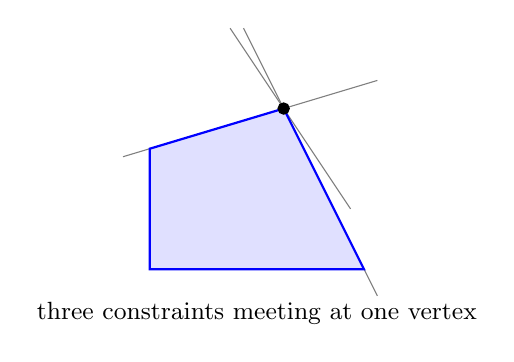
\begin{tikzpicture}[scale=0.85]
    \fill[color=blue!12] (0,0) -- (3.2,0) -- (2.0,2.4) -- (0,1.8) -- cycle;
    % the three constraint lines, extended beyond the vertex
    \draw[thin, color=gray] (3.4,-0.4) -- (1.4,3.6);
    \draw[thin, color=gray] (-0.4,1.68) -- (3.4,2.82);
    \draw[thin, color=gray] (1.2,3.6) -- (3.0,0.9);
    \draw[thick, color=blue] (0,0) -- (3.2,0) -- (2.0,2.4) -- (0,1.8) -- cycle;
    \filldraw (2.0,2.4) circle (2.4pt);
    \node[anchor=north] at (1.6,-0.35) {\small three constraints meeting at one vertex};
\end{tikzpicture}
\end{center}

If the ratio test is a tie, then $\theta^*$ may be zero: the pivot changes the basis but does \emph{not} move the point. The cost then does not decrease, and it becomes possible in principle for the algorithm to return to a basis it has already visited, and loop forever. This is called \vocab{cycling}. It is rare in practice but it genuinely happens, and there are small explicit examples.

The fix is to break ties in a way that provably cannot cycle.

\begin{definition}[Bland's Rule]
    \vocab{Bland's rule} is to resolve both choices in the simplex method by smallest index:
    \begin{enumerate}[label=(\roman*)]
        \item among all $j$ with $\bar c_j < 0$, choose the pivot column with the smallest index $j$;
        \item among all rows attaining the minimum in the ratio test, choose the one whose \emph{basic variable} $B(\ell)$ has the smallest index.
    \end{enumerate}
\end{definition}

\begin{theorem}[Bland]
    The simplex method with Bland's rule terminates.
\end{theorem}
\begin{proof}[Proof sketch]
    Suppose the algorithm cycles. During a cycle the cost never changes, so every pivot has $\theta^* = 0$ and the point $x$ is fixed throughout; let $D$ be the set of variables that enter and leave the basis during the cycle, and let $q$ be the largest index in $D$. Consider the iteration at which $q$ leaves the basis, say with entering variable $p \in D$ (so $p < q$), and the (later) iteration at which $q$ enters. One shows by comparing the reduced costs at these two iterations that the choice of $p$ at the first iteration and the choice of $q$ at the second are inconsistent with the smallest-index rule: at the second iteration the variable $p$ would still have had negative reduced cost, and $p < q$, so $p$ would have been chosen instead of $q$. This contradiction shows no cycle can occur, and since there are finitely many bases the algorithm terminates.
\end{proof}

An alternative and more common fix in practice is \emph{lexicographic} pivoting, which amounts to perturbing $b$ to $b + (\varepsilon, \varepsilon^2, \dots, \varepsilon^m)$ for a formal infinitesimal $\varepsilon$, thereby making every basic solution non-degenerate.

\begin{remark}[How fast is the simplex method?]
    We have shown that the simplex method terminates, but the bound we get is terrible: there are $\binom nm$ bases and in principle we might visit a large fraction of them. In fact Klee and Minty constructed, for each $n$, a linear program on a slightly squashed $n$-dimensional cube for which Dantzig's original pivoting rule visits all $2^n$ vertices. So the simplex method is not a polynomial-time algorithm, at least for that rule, and no pivoting rule is known to be polynomial.

    Nevertheless the simplex method is superb in practice: on real problems it typically takes a number of pivots linear in $m$, and this behaviour can be made precise in various average-case and smoothed-analysis models. Meanwhile there \emph{are} provably polynomial-time algorithms for linear programming -- the ellipsoid method of Khachiyan and the interior point methods descended from Karmarkar's algorithm, which are essentially the barrier methods of Section 1.4 applied to linear constraints. Modern solvers implement both families and choose between them.
\end{remark}

\subsection{The Two-Phase Simplex Method}

There is one loose end: the simplex method has to start at a basic feasible solution, and in the example above we were handed one by the slack variables. That is a piece of luck peculiar to problems of the form $Ax \leq b$ with $b \geq 0$. In general -- for instance with $\geq$ constraints, where the surplus variables would need to be negative -- finding an initial bfs is itself a non-trivial problem.

The trick is that finding a feasible point is itself a linear program that we can solve by the simplex method, and \emph{that} problem always has an obvious starting point. We introduce \vocab{artificial variables}.

Given the standard-form problem `minimize $c\cdot x$ subject to $Ax = b$, $x \geq 0$', where without loss of generality $b \geq 0$ (multiply rows by $-1$ if needed), consider the auxiliary problem
\begin{alignat*}{2}
    & \text{minimize} \quad && y_1 + \cdots + y_m \\
    & \text{subject to} \quad && Ax + y = b, \\
    & && x, y \geq 0.
\end{alignat*}
This has the obvious basic feasible solution $x = 0$, $y = b$. Moreover its optimal value is $0$ if and only if the original problem is feasible, and any solution with $y = 0$ gives a feasible $x$. So:
\begin{itemize}
    \item \textbf{Phase I:} solve the auxiliary problem by the simplex method. If the optimal value is positive, the original problem is infeasible and we stop. Otherwise we finish with a basic feasible solution in which all the artificial variables are zero.
    \item \textbf{Phase II:} drop the artificial variables and the Phase I objective row, and run the simplex method on the original objective starting from the basis just found.
\end{itemize}

In practice we carry both objective rows through Phase I, so that the original objective row is correctly updated and ready for Phase II.

\begin{example}
    Consider
    \begin{alignat*}{2}
        & \text{minimize} \quad && 6x_1 + 3x_2 \\
        & \text{subject to} \quad && x_1 + x_2 \geq 1, \\
        & && 2x_1 - x_2 \geq 1, \\
        & && 3x_2 \leq 2, \\
        & && x_1, x_2 \geq 0.
    \end{alignat*}
    Adding surplus variables $z_1, z_2$ and a slack $z_3$,
    $$
    x_1 + x_2 - z_1 = 1, \quad 2x_1 - x_2 - z_2 = 1, \quad 3x_2 + z_3 = 2.
    $$
    Setting $x = 0$ would force $z_1 = z_2 = -1$, which is infeasible, so we add artificial variables $y_1, y_2$ to the first two rows and minimize $y_1 + y_2$. The starting basis is $\{y_1, y_2, z_3\}$, giving the tableau (with the original objective in row $0$ and the Phase I objective in row $0'$):
    $$
    \arraycolsep=5pt\def\arraystretch{1.3}
    \begin{array}{|c|ccccccc|}\hline
        \multicolumn{1}{|c|}{} & x_1 & x_2 & z_1 & z_2 & z_3 & y_1 & y_2\\\hline
        0 & 6 & 3 & 0 & 0 & 0 & 0 & 0\\
        0 & 0 & 0 & 0 & 0 & 0 & 1 & 1\\\hline
        1 & 1 & 1 & -1 & 0 & 0 & 1 & 0\\
        1 & 2 & -1 & 0 & -1 & 0 & 0 & 1\\
        2 & 0 & 3 & 0 & 0 & 1 & 0 & 0\\\hline
    \end{array}
    $$
    This is not yet a valid tableau, because the reduced costs in the basic columns $y_1, y_2$ must be zero. Subtracting rows $1$ and $2$ from row $0'$ fixes this:
    $$
    \arraycolsep=5pt\def\arraystretch{1.3}
    \begin{array}{|c|ccccccc|}\hline
        \multicolumn{1}{|c|}{} & x_1 & x_2 & z_1 & z_2 & z_3 & y_1 & y_2\\\hline
        0 & 6 & 3 & 0 & 0 & 0 & 0 & 0\\
        -2 & -3 & 0 & 1 & 1 & 0 & 0 & 0\\\hline
        1 & 1 & 1 & -1 & 0 & 0 & 1 & 0\\
        1 & \boxed{2} & -1 & 0 & -1 & 0 & 0 & 1\\
        2 & 0 & 3 & 0 & 0 & 1 & 0 & 0\\\hline
    \end{array}
    $$
    The Phase I cost is $2$ (top-left of row $0'$ is $-2$). Pivoting on the boxed entry in column $x_1$ (ratios $1/1 = 1$ and $1/2 = \frac12$, the latter smaller):
    $$
    \arraycolsep=5pt\def\arraystretch{1.3}
    \begin{array}{|c|ccccccc|}\hline
        \multicolumn{1}{|c|}{} & x_1 & x_2 & z_1 & z_2 & z_3 & y_1 & y_2\\\hline
        -3 & 0 & 6 & 0 & 3 & 0 & 0 & -3\\
        -\frac12 & 0 & -\frac32 & 1 & -\frac12 & 0 & 0 & \frac32\\\hline
        \frac12 & 0 & \boxed{\tfrac32} & -1 & \frac12 & 0 & 1 & -\frac12\\
        \frac12 & 1 & -\frac12 & 0 & -\frac12 & 0 & 0 & \frac12\\
        2 & 0 & 3 & 0 & 0 & 1 & 0 & 0\\\hline
    \end{array}
    $$
    Now $\bar c_{x_2} = -\frac32 < 0$ in the Phase I row. The ratios are $\frac12 / \frac32 = \frac13$ and $2/3$, so we pivot on the boxed $\frac32$:
    $$
    \arraycolsep=5pt\def\arraystretch{1.3}
    \begin{array}{|c|ccccccc|}\hline
        \multicolumn{1}{|c|}{} & x_1 & x_2 & z_1 & z_2 & z_3 & y_1 & y_2\\\hline
        -5 & 0 & 0 & 4 & 1 & 0 & -4 & -1\\
        0 & 0 & 0 & 0 & 0 & 0 & 1 & 1\\\hline
        \frac13 & 0 & 1 & -\frac23 & \frac13 & 0 & \frac23 & -\frac13\\
        \frac23 & 1 & 0 & -\frac13 & -\frac13 & 0 & \frac13 & \frac13\\
        1 & 0 & 0 & 2 & -1 & 1 & -2 & 1\\\hline
    \end{array}
    $$
    The Phase I objective is now $0$ and the artificial variables have left the basis, so Phase I is complete. Deleting the artificial columns and the Phase I row leaves
    $$
    \arraycolsep=5pt\def\arraystretch{1.3}
    \begin{array}{|c|ccccc|}\hline
        \multicolumn{1}{|c|}{} & x_1 & x_2 & z_1 & z_2 & z_3\\\hline
        -5 & 0 & 0 & 4 & 1 & 0\\\hline
        \frac13 & 0 & 1 & -\frac23 & \frac13 & 0\\
        \frac23 & 1 & 0 & -\frac13 & -\frac13 & 0\\
        1 & 0 & 0 & 2 & -1 & 1\\\hline
    \end{array}
    $$
    All reduced costs in row $0$ are non-negative, so we are already optimal -- Phase II has nothing to do. The optimal solution is $x_1 = \frac23$, $x_2 = \frac13$, $z_3 = 1$, with optimal cost $6\cdot\frac23 + 3\cdot\frac13 = 5$, which is consistent with the top-left entry $-5$.
\end{example}

\begin{remark}
    It can happen that Phase I terminates with optimal value $0$ but with an artificial variable still in the basis (at value zero). This is a degenerate situation; one can always pivot it out on any nonzero entry in a non-artificial column, or if the whole row is zero, delete the row as redundant.
\end{remark}

\subsection{The Dual Simplex Method}

The simplex method as described maintains primal feasibility and complementary slackness at every step, and works towards dual feasibility. There is a mirror-image algorithm, the \vocab{dual simplex method}, which maintains \emph{dual} feasibility and complementary slackness and works towards primal feasibility. In tableau terms: we start with a tableau whose row $0$ is non-negative but whose left-hand column has some negative entries, and we pivot to remove the negative entries while keeping row $0$ non-negative.

\begin{definition}[Dual Simplex Method]
    Given a tableau with $\bar c \geq 0$:
    \begin{enumerate}[label=(\arabic*)]
        \item If $B^{-1}b \geq 0$, stop: the solution is primal feasible, and hence optimal.
        \item Otherwise choose a \vocab{pivot row} $\ell$ with $(B^{-1}b)_\ell < 0$.
        \item If every entry of row $\ell$ (in the body) is non-negative, stop: the primal is infeasible.
        \item Otherwise choose the \vocab{pivot column} $j$ minimizing $\left|\bar c_j / a_{\ell j}\right|$ over all $j$ with $a_{\ell j} < 0$.
        \item Pivot on the entry $a_{\ell j}$ as usual, and go to (1).
    \end{enumerate}
\end{definition}

The ratio test in step (4) is exactly what is needed to keep row $0$ non-negative: after pivoting, $\bar c_k$ becomes $\bar c_k - (\bar c_j / a_{\ell j})a_{\ell k}$, and one checks that the minimizing choice keeps all of these non-negative. Notice that the roles of rows and columns, and of the two feasibility conditions, have swapped relative to the primal simplex method -- which is precisely what one would expect from the fact that the dual of the dual is the primal.

The dual simplex method is extremely useful when we have already solved a problem and then change $b$ (for instance by adding a new constraint). The old solution stays dual feasible but may become primal infeasible, so we can restart from it with the dual simplex method rather than solving from scratch.

\begin{example}
    Consider
    \begin{alignat*}{2}
        & \text{minimize} \quad && 2x_1 + 3x_2 \\
        & \text{subject to} \quad && x_1 + x_2 \geq 2, \\
        & && x_1 + 3x_2 \geq 3, \\
        & && x_1, x_2 \geq 0.
    \end{alignat*}
    Subtracting surplus variables and then multiplying both constraint rows by $-1$ to make the slack variables basic, we get $-x_1 - x_2 + z_1 = -2$ and $-x_1 - 3x_2 + z_2 = -3$ with $z_1, z_2 \geq 0$, and the basis $\{z_1, z_2\}$ gives the tableau
    $$
    \arraycolsep=6pt\def\arraystretch{1.3}
    \begin{array}{|c|cccc|}\hline
        \multicolumn{1}{|c|}{} & x_1 & x_2 & z_1 & z_2\\\hline
        0 & 2 & 3 & 0 & 0\\\hline
        -2 & -1 & -1 & 1 & 0\\
        -3 & -1 & \boxed{-3} & 0 & 1\\\hline
    \end{array}
    $$
    Row $0$ is non-negative (dual feasible) but the left column is not (primal infeasible), so we use the dual simplex method. The most negative entry is $-3$ in row $2$, so we take $\ell = 2$. The ratios $|\bar c_j/a_{2j}|$ for the negative entries of that row are $|2/(-1)| = 2$ and $|3/(-3)| = 1$, so we pivot on the boxed $-3$ in column $x_2$:
    $$
    \arraycolsep=6pt\def\arraystretch{1.3}
    \begin{array}{|c|cccc|}\hline
        \multicolumn{1}{|c|}{} & x_1 & x_2 & z_1 & z_2\\\hline
        -3 & 1 & 0 & 0 & 1\\\hline
        -1 & \boxed{-\tfrac23} & 0 & 1 & -\frac13\\
        1 & \frac13 & 1 & 0 & -\frac13\\\hline
    \end{array}
    $$
    Still one negative entry in the left column, so $\ell = 1$. The negative entries in that row are $-\frac23$ in column $x_1$ and $-\frac13$ in column $z_2$, with ratios $|1/(-\frac23)| = \frac32$ and $|1/(-\frac13)| = 3$; so we pivot on the boxed $-\frac23$:
    $$
    \arraycolsep=6pt\def\arraystretch{1.3}
    \begin{array}{|c|cccc|}\hline
        \multicolumn{1}{|c|}{} & x_1 & x_2 & z_1 & z_2\\\hline
        -\frac92 & 0 & 0 & \frac32 & \frac12\\\hline
        \frac32 & 1 & 0 & -\frac32 & \frac12\\
        \frac12 & 0 & 1 & \frac12 & -\frac12\\\hline
    \end{array}
    $$
    Now both the left column and row $0$ are non-negative, so we have an optimal solution $x^* = (\frac32, \frac12)$ with optimal cost $\frac92$. Note that we never needed a Phase I.
\end{example}

\section{Network Problems}

A great many of the linear programs that arise in practice have a very particular shape: the variables are indexed by the edges of a graph, and the constraints say that whatever flows into a vertex must flow out of it again. These are the \vocab{network flow} problems. They are important both because they model an enormous range of real situations -- shipping goods, routing traffic, scheduling, matching -- and because their special structure lets us solve them far more efficiently than by general-purpose simplex.

\subsection{Flows in Networks}

\begin{definition}[Directed Graph]
    A \vocab{directed graph} (or \vocab{digraph}) is a pair $G = (V, E)$ where $V$ is a finite set of \vocab{vertices} and $E \subseteq V \times V$ is a set of \vocab{edges}. We think of $(i,j) \in E$ as an arrow from $i$ to $j$.
\end{definition}

\begin{definition}[Flow]
    Let $G = (V,E)$ be a digraph on $n$ vertices. A \vocab{flow} on $G$ is an assignment of a real number $x_{ij}$ to each edge $(i,j) \in E$, thought of as the amount of some commodity travelling along that edge. The flow is subject to:
    \begin{itemize}
        \item a vector $b \in \R^n$, where $b_i$ is the amount injected into the network at vertex $i$ from outside. If $b_i > 0$ we call $i$ a \vocab{source} and if $b_i < 0$ a \vocab{sink};
        \item a \vocab{cost} $c_{ij}$ per unit of flow along $(i,j)$;
        \item capacities $\underline m_{ij} \leq x_{ij} \leq \overline m_{ij}$ on each edge.
    \end{itemize}
\end{definition}

\begin{definition}[Minimum Cost Flow]
    The \vocab{minimum cost flow problem} is the linear program
    \begin{alignat*}{2}
        & \text{minimize} \quad && \sum_{(i,j) \in E}c_{ij}x_{ij} \\
        & \text{subject to} \quad && b_i + \sum_{j\,:\,(j,i)\in E}x_{ji} = \sum_{j\,:\,(i,j)\in E}x_{ij} \quad \text{ for all } i \in V,\\
        & && \underline m_{ij} \leq x_{ij} \leq \overline m_{ij} \quad \text{ for all } (i,j) \in E.
    \end{alignat*}
    The first family of constraints is \vocab{conservation of flow}: what goes in must come out.
\end{definition}

Summing the conservation equations over all $i$, every $x_{ij}$ appears once on each side, so we get $\sum_i b_i = 0$. This is a necessary condition for feasibility, and it is obvious: the network has no storage, so the total injected must equal the total removed.

The conservation constraints can be written compactly.

\begin{definition}[Incidence Matrix]
    The \vocab{incidence matrix} of $G$ is the matrix $A \in \R^{|V|\times|E|}$ whose column indexed by the edge $(i,j)$ has $+1$ in row $i$, $-1$ in row $j$, and zeros elsewhere.
\end{definition}

With this notation the conservation constraints are exactly $Ax = b$, and the minimum cost flow problem is a linear program in the (almost) standard form we have been studying. What makes network problems special is that $A$ is a very sparse matrix with entries in $\{0, \pm 1\}$, and this has strong consequences -- notably, if $b$ and the capacities are integers then there is an integral optimal solution.

\subsection{The Transportation Problem}

The most important special case is when the graph is bipartite.

\begin{definition}[Transportation Problem]
    Suppose we have $n$ suppliers, where supplier $i$ has $s_i$ units available, and $m$ consumers, where consumer $j$ demands $d_j$ units, with $\sum_i s_i = \sum_j d_j$. Shipping one unit from $i$ to $j$ costs $c_{ij}$. The \vocab{transportation problem} is
    \begin{alignat*}{2}
        & \text{minimize} \quad && \sum_{i=1}^n\sum_{j=1}^m c_{ij}x_{ij} \\
        & \text{subject to} \quad && \sum_{j=1}^m x_{ij} = s_i \quad\text{ for } i = 1, \dots, n,\\
        & && \sum_{i=1}^n x_{ij} = d_j \quad\text{ for } j = 1, \dots, m,\\
        & && x \geq 0.
    \end{alignat*}
\end{definition}

\begin{center}
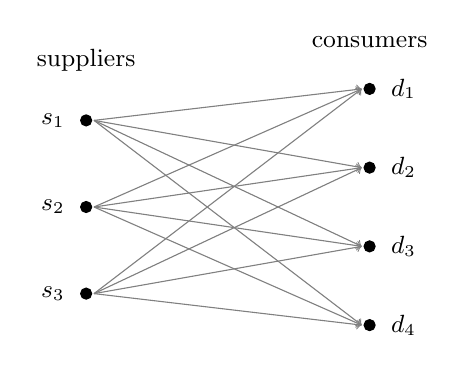
\begin{tikzpicture}[scale=1.0]
    \foreach \i/\y/\lab in {1/2.2/{s_1}, 2/1.1/{s_2}, 3/0.0/{s_3}} {
        \filldraw (0,\y) circle (2.0pt);
        \node[anchor=east] at (-0.15,\y) {\small $\lab$};
    }
    \foreach \j/\y/\lab in {1/2.6/{d_1}, 2/1.6/{d_2}, 3/0.6/{d_3}, 4/-0.4/{d_4}} {
        \filldraw (3.6,\y) circle (2.0pt);
        \node[anchor=west] at (3.75,\y) {\small $\lab$};
    }
    \foreach \sy in {2.2, 1.1, 0.0} {
        \foreach \dy in {2.6, 1.6, 0.6, -0.4} {
            \draw[->, thin, color=gray] (0.1,\sy) -- (3.5,\dy);
        }
    }
    \node[anchor=south] at (0,2.7) {\small suppliers};
    \node[anchor=south] at (3.6,3.0) {\small consumers};
\end{tikzpicture}
\end{center}

This looks like a special case, but it is in fact completely general.

\begin{theorem}
    Every minimum cost flow problem with finite capacities, or with non-negative costs, is equivalent to a transportation problem.
\end{theorem}
\begin{proof}
    First we normalize. We may assume $\underline m_{ij} = 0$ for all edges: substituting $x_{ij} = \underline m_{ij} + \tilde x_{ij}$ turns the constraint into $0 \leq \tilde x_{ij} \leq \overline m_{ij} - \underline m_{ij}$ and the conservation equations into the same equations with
    $$
    \tilde b_i = b_i + \sum_{j\,:\,(j,i)\in E}\underline m_{ji} - \sum_{j\,:\,(i,j)\in E}\underline m_{ij}.
    $$
    (We are just secretly shipping the minimum amount along each edge before we start.) Next, if some capacity is infinite but all costs are non-negative, we may replace it by $\sum_i|b_i|$, since no optimal solution ever ships more than this along any edge (it would have to run round a cycle, and cycles cost nothing to remove when costs are non-negative). So assume all capacities are finite.

    Now build a transportation problem. For each \emph{vertex} $i$ of the original graph, create a consumer with demand
    $$
    \sum_{k\,:\,(i,k)\in E}\overline m_{ik} - b_i.
    $$
    For each \emph{edge} $(i,j)$ of the original graph, create a supplier with supply $\overline m_{ij}$, joined to consumer $i$ at cost $0$ and to consumer $j$ at cost $c_{ij}$.
\begin{center}
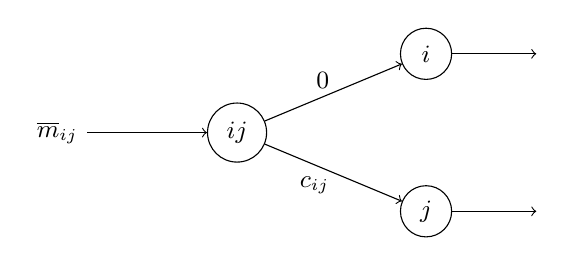
\begin{tikzpicture}[scale=1.0]
    \node[draw, circle, inner sep=1pt, minimum width=0.75cm] (ij) at (0,0) {\small $ij$};
    \node[draw, circle, inner sep=1pt, minimum width=0.65cm] (i) at (2.4,1.0) {\small $i$};
    \node[draw, circle, inner sep=1pt, minimum width=0.65cm] (j) at (2.4,-1.0) {\small $j$};
    \draw[->] (ij) -- (i) node[pos=0.5, above left=-2pt] {\small $0$};
    \draw[->] (ij) -- (j) node[pos=0.5, below left=-2pt] {\small $c_{ij}$};
    \draw[->] (-1.9,0) node[anchor=east] {\small $\overline m_{ij}$} -- (ij);
    \draw[->] (i) -- +(1.4,0);
    \draw[->] (j) -- +(1.4,0);
\end{tikzpicture}
\end{center}
    Total supply is $\sum_{(i,j)}\overline m_{ij}$, and total demand is $\sum_i\left(\sum_k \overline m_{ik} - b_i\right) = \sum_{(i,j)}\overline m_{ij}$ since $\sum_i b_i = 0$; so the transportation problem is balanced.

    Given a flow $x$ in the original network, ship $x_{ij}$ from supplier $(i,j)$ to consumer $j$ and the remaining $\overline m_{ij} - x_{ij}$ to consumer $i$. Then supplier $(i,j)$'s supply is exactly used up, and $0 \leq x_{ij} \leq \overline m_{ij}$ is exactly the requirement that both shipments are non-negative. The total received by consumer $i$ is
    $$
    \sum_{k\,:\,(i,k)\in E}(\overline m_{ik} - x_{ik}) + \sum_{k\,:\,(k,i)\in E}x_{ki},
    $$
    and setting this equal to the demand $\sum_k \overline m_{ik} - b_i$ rearranges precisely to the conservation equation at $i$. Finally, the cost of the transportation solution is $\sum_{(i,j)}c_{ij}x_{ij}$, since the edges into consumer $i$ are free. So the two problems are equivalent.
\end{proof}

\subsection{Optimality for the Transportation Problem}

The transportation problem is a linear program, so we know exactly what optimality means: primal feasibility, dual feasibility and complementary slackness. Let us compute what these say. Since there are two families of constraints, we take two families of multipliers: $\lambda \in \R^n$ for the suppliers and $\mu \in \R^m$ for the consumers. The Lagrangian is
\begin{align*}
    L(x,\lambda,\mu) &= \sum_{i,j}c_{ij}x_{ij} - \sum_{i}\lambda_i\left(\sum_j x_{ij} - s_i\right) - \sum_j\mu_j\left(\sum_i x_{ij} - d_j\right)\\
    &= \sum_{i,j}\left(c_{ij} - \lambda_i - \mu_j\right)x_{ij} + \sum_i\lambda_i s_i + \sum_j\mu_j d_j.
\end{align*}
Since $x \geq 0$, this has a finite infimum exactly when $c_{ij} - \lambda_i - \mu_j \geq 0$ for all $i,j$.

\begin{theorem}[Optimality Conditions]
    A feasible $x$ is optimal for the transportation problem if there exist $\lambda \in \R^n$, $\mu \in \R^m$ with
    \begin{enumerate}[label=(\roman*)]
        \item $\lambda_i + \mu_j \leq c_{ij}$ for all $(i,j)$ \hfill (dual feasibility)
        \item $\left(c_{ij} - \lambda_i - \mu_j\right)x_{ij} = 0$ for all $(i,j)$ \hfill (complementary slackness)
    \end{enumerate}
\end{theorem}
\begin{proof}
    Immediate from the general optimality conditions for a linear program, applied to the Lagrangian above.
\end{proof}

Condition (ii) says: wherever we actually ship something, the dual constraint is tight. Note that the multipliers are not unique -- adding a constant $k$ to every $\lambda_i$ and subtracting it from every $\mu_j$ changes nothing. We therefore normalize by setting $\lambda_1 = 0$, which leaves $m + n - 1$ unknowns.

To get started we need an initial basic feasible solution, and here there is a very simple recipe: the \vocab{north-west corner rule}. Start at the top-left cell of the table, ship as much as possible (the smaller of the remaining supply and remaining demand), cross off whichever of the row or column is exhausted, and repeat.

\begin{theorem}
    The set of cells with $x_{ij} > 0$ in a basic feasible solution of the transportation problem forms a spanning tree of the bipartite graph, and hence contains exactly $m + n - 1$ cells.
\end{theorem}

We will not prove this, but it is easy to believe: there are $m + n$ constraints of which one is redundant (because $\sum s_i = \sum d_j$), so a basis has $m + n - 1$ elements; and a set of edges with no cycle and $m+n-1$ elements on $m+n$ vertices is a spanning tree. The practical consequence is that the equations $\lambda_i + \mu_j = c_{ij}$ over the basic cells, together with $\lambda_1 = 0$, always have a unique solution -- we can propagate along the tree.

\subsection{The Transportation Algorithm}

We record the data in a \vocab{transportation tableau}, one cell per $(i,j)$, showing the current flow $x_{ij}$, the cost $c_{ij}$ and the quantity $\lambda_i + \mu_j$, with the supplies down the right, the demands along the bottom, and $\lambda, \mu$ in the margins. The algorithm is then:
\begin{enumerate}[label=(\arabic*)]
    \item Find an initial basic feasible solution (e.g.\ by the north-west corner rule).
    \item Solve $\lambda_i + \mu_j = c_{ij}$ over the basic cells, with $\lambda_1 = 0$.
    \item If $\lambda_i + \mu_j \leq c_{ij}$ for every cell, stop -- the solution is optimal.
    \item Otherwise pick a cell $(i,j)$ with $\lambda_i + \mu_j > c_{ij}$. Adding $(i,j)$ to the spanning tree creates a unique cycle. Send $\theta$ units around this cycle (alternately $+\theta$ and $-\theta$), increasing $\theta$ until some basic cell is driven to zero. That cell leaves the basis and $(i,j)$ enters.
    \item Go to (2).
\end{enumerate}
This is exactly the simplex method in disguise: step (3) is the check $\bar c \geq 0$, and step (4) is the ratio test.

\begin{example}
    Take three suppliers with $s = (14, 10, 9)$ and four consumers with $d = (12,5,8,8)$, and costs
    $$
    C = \begin{pmatrix} 5 & 3 & 4 & 6\\ 2 & 7 & 4 & 1\\ 5 & 6 & 2 & 4\end{pmatrix}.
    $$
    The north-west corner rule gives
    $$
    x = \begin{pmatrix}12 & 2 & 0 & 0\\ 0 & 3 & 7 & 0\\0&0&1&8\end{pmatrix},
    $$
    with basic cells $(1,1),(1,2),(2,2),(2,3),(3,3),(3,4)$ -- six of them, as promised. Complementary slackness gives
    $$
    \lambda_1 + \mu_1 = 5,\quad \lambda_1 + \mu_2 = 3,\quad \lambda_2 + \mu_2 = 7,\quad \lambda_2 + \mu_3 = 4,\quad \lambda_3+\mu_3 = 2,\quad \lambda_3 + \mu_4 = 4,
    $$
    which with $\lambda_1 = 0$ solves to
    $$
    \lambda = (0, 4, 2), \qquad \mu = (5, 3, 0, 2).
    $$
    It is convenient to record all of this in a single tableau, with the multipliers in the margins and each cell showing the current flow and the cost, written $x_{ij}\,|\,c_{ij}$:
    \begin{center}
    \begin{tabular}{r|cccc|c}
        & $\mu_1 = 5$ & $\mu_2 = 3$ & $\mu_3 = 0$ & $\mu_4 = 2$ & $s_i$\\\hline
        $\lambda_1 = 0$ & $12\,|\,5$ & $2\,|\,3$ & $0\,|\,4$ & $0\,|\,6$ & $14$\\
        $\lambda_2 = 4$ & $0\,|\,2$ & $3\,|\,7$ & $7\,|\,4$ & $0\,|\,1$ & $10$\\
        $\lambda_3 = 2$ & $0\,|\,5$ & $0\,|\,6$ & $1\,|\,2$ & $8\,|\,4$ & $9$\\\hline
        $d_j$ & $12$ & $5$ & $8$ & $8$ &
    \end{tabular}
    \end{center}
    One checks at a glance that the rows sum to the supplies and the columns to the demands. Now we tabulate $\lambda_i + \mu_j$ against $c_{ij}$:
    $$
    \arraycolsep=6pt\def\arraystretch{1.3}
    \begin{array}{c|cccc}
        \lambda_i + \mu_j & \mu_1 = 5 & \mu_2 = 3 & \mu_3 = 0 & \mu_4 = 2\\\hline
        \lambda_1 = 0 & 5\ (5) & 3\ (3) & 0\ (4) & 2\ (6)\\
        \lambda_2 = 4 & \mathbf{9}\ (2) & 7\ (7) & 4\ (4) & 6\ (1)\\
        \lambda_3 = 2 & 7\ (5) & 5\ (6) & 2\ (2) & 4\ (4)
    \end{array}
    $$
    (costs $c_{ij}$ in brackets). Cell $(2,1)$ violates the condition badly: $9 > 2$. Cell $(2,4)$ also violates it, as does $(3,1)$; we pick $(2,1)$.

    Adding $(2,1)$ to the tree creates the cycle $(2,1) \rightarrow (1,1) \rightarrow (1,2) \rightarrow (2,2) \rightarrow (2,1)$. Putting $\theta$ into $(2,1)$ forces $x_{11} \mapsto 12 - \theta$, $x_{12}\mapsto 2 + \theta$ and $x_{22}\mapsto 3 - \theta$. The binding constraint is $x_{22} \geq 0$, so $\theta = 3$ and cell $(2,2)$ leaves. The new solution is
    $$
    x = \begin{pmatrix}9 & 5 & 0 & 0\\3&0&7&0\\0&0&1&8\end{pmatrix},
    $$
    with basic cells $(1,1),(1,2),(2,1),(2,3),(3,3),(3,4)$. Re-solving for the multipliers,
    $$
    \lambda_1 + \mu_1 = 5,\ \lambda_1+\mu_2 = 3,\ \lambda_2 + \mu_1 = 2,\ \lambda_2 + \mu_3 = 4,\ \lambda_3 + \mu_3 = 2,\ \lambda_3+\mu_4 = 4,
    $$
    giving $\lambda = (0,-3,-5)$ and $\mu = (5,3,7,9)$. Checking again:
    $$
    \arraycolsep=6pt\def\arraystretch{1.3}
    \begin{array}{c|cccc}
        \lambda_i + \mu_j & \mu_1 = 5 & \mu_2 = 3 & \mu_3 = 7 & \mu_4 = 9\\\hline
        \lambda_1 = 0 & 5\ (5) & 3\ (3) & 7\ (4) & 9\ (6)\\
        \lambda_2 = -3 & 2\ (2) & 0\ (7) & 4\ (4) & \mathbf{6}\ (1)\\
        \lambda_3 = -5 & 0\ (5) & -2\ (6) & 2\ (2) & 4\ (4)
    \end{array}
    $$
    Now $(2,4)$ violates: $6 > 1$. (So does $(1,3)$ and $(1,4)$.) Taking $(2,4)$, the cycle is $(2,4)\rightarrow(2,3)\rightarrow(3,3)\rightarrow(3,4)\rightarrow(2,4)$, so $x_{23}\mapsto 7 - \theta$, $x_{33}\mapsto 1 + \theta$, $x_{34}\mapsto 8 - \theta$. The binding constraint is $x_{23} \geq 0$ at $\theta = 7$, giving
    $$
    x = \begin{pmatrix}9&5&0&0\\3&0&0&7\\0&0&8&1\end{pmatrix}.
    $$
    The new multipliers solve to $\lambda = (0,-3,0)$ and $\mu = (5,3,2,4)$, and now
    $$
    \arraycolsep=6pt\def\arraystretch{1.3}
    \begin{array}{c|cccc}
        \lambda_i + \mu_j & \mu_1 = 5 & \mu_2 = 3 & \mu_3 = 2 & \mu_4 = 4\\\hline
        \lambda_1 = 0 & 5\ (5) & 3\ (3) & 2\ (4) & 4\ (6)\\
        \lambda_2 = -3 & 2\ (2) & 0\ (7) & -1\ (4) & 1\ (1)\\
        \lambda_3 = 0 & 5\ (5) & 3\ (6) & 2\ (2) & 4\ (4)
    \end{array}
    $$
    Every entry satisfies $\lambda_i + \mu_j \leq c_{ij}$, so we are optimal. The cost is
    $$
    9\cdot 5 + 5\cdot 3 + 3\cdot 2 + 7\cdot 1 + 8\cdot 2 + 1\cdot 4 = 45+15+6+7+16+4 = 93.
    $$
\end{example}

\begin{remark}[Transshipment]
    A variant that often occurs is the \vocab{transshipment problem}, in which goods may pass through intermediate depots rather than going directly from supplier to consumer. Formally this is just a minimum cost flow problem on a graph with some vertices having $b_i = 0$, and by the reduction theorem above it can be converted into a transportation problem. In practice a slicker route is available: replace each cost $c_{ij}$ by the cost $\hat c_{ij}$ of the \emph{cheapest path} from $i$ to $j$ in the network (computable by any shortest-path algorithm), and then solve the resulting transportation problem with costs $\hat c$. Any optimal solution of that problem is realized by routing each shipment along its cheapest path.
\end{remark}

\subsection{The Assignment Problem}

A further special case, and one of the classics, is the following.

\begin{definition}[Assignment Problem]
    Given $n$ workers and $n$ jobs, and a cost $c_{ij}$ of assigning worker $i$ to job $j$, the \vocab{assignment problem} is to find a bijection $\sigma$ from workers to jobs minimizing $\sum_i c_{i\sigma(i)}$.
\end{definition}

Written as an optimization over $\{0,1\}$-matrices this is a combinatorial problem with $n!$ candidates, which sounds hopeless. But it is exactly a transportation problem with $s_i = d_j = 1$ for all $i, j$:
\begin{alignat*}{2}
    & \text{minimize} \quad && \sum_{i,j}c_{ij}x_{ij} \\
    & \text{subject to} \quad && \textstyle\sum_j x_{ij} = 1 \text{ for each } i,\quad \sum_i x_{ij} = 1 \text{ for each } j,\quad x \geq 0.
\end{alignat*}
The feasible set of this linear program consists of the \emph{doubly stochastic} matrices, and the corresponding combinatorial problem is recovered by the following classical fact, which we quote.

\begin{theorem}[Birkhoff--von Neumann]
    The extreme points of the set of doubly stochastic $n \times n$ matrices are exactly the permutation matrices.
\end{theorem}

Combining this with the fundamental theorem of linear programming, some optimal solution of the linear program is an extreme point, hence a permutation matrix, hence an honest assignment. So we may simply solve the transportation problem and read off the answer -- an $n!$-sized search has been replaced by a polynomial-time algorithm. This phenomenon, where the linear relaxation of an integer problem automatically has integral optima, is exactly what makes network problems so tractable, and it recurs in the maximum flow problem below.

\subsection{The Maximum Flow Problem}

We now turn to a different, and in some ways more fundamental, network problem. There are no costs; instead every edge has a capacity, there is a single source (vertex $1$) and a single sink (vertex $n$), and we want to push as much as possible from source to sink.

\begin{definition}[Maximum Flow Problem]
    Given a digraph $G = (V,E)$ on vertices $\{1, \dots, n\}$ with capacities $c_{ij} \geq 0$, the \vocab{maximum flow problem} is
    \begin{alignat*}{2}
        & \text{maximize} \quad && \delta \\
        & \text{subject to} \quad && \sum_{j\,:\,(i,j)\in E}x_{ij} - \sum_{j\,:\,(j,i)\in E}x_{ji} = \begin{cases}\delta & i = 1\\ -\delta & i = n\\ 0 & \text{otherwise},\end{cases}\\
        & && 0 \leq x_{ij} \leq c_{ij} \quad \text{ for all } (i,j)\in E.
    \end{alignat*}
    We call $\delta$ the \vocab{value} of the flow.
\end{definition}

This is a minimum cost flow problem in disguise: add an edge from $n$ back to $1$ with cost $-1$ and infinite capacity, and set all $b_i = 0$; then minimizing the cost is the same as maximizing the flow round the added edge, which is $\delta$. But there is a much better way to think about it.

\begin{definition}[Cut]
    A \vocab{cut} of $G$ is a partition of $V$ into two sets $(S, V\setminus S)$. Its \vocab{capacity} is
    $$
    C(S) = \sum_{\substack{(i,j) \in E \\ i \in S,\ j \in V\setminus S}} c_{ij},
    $$
    the total capacity of the edges crossing from $S$ to $V\setminus S$.
\end{definition}

\begin{center}
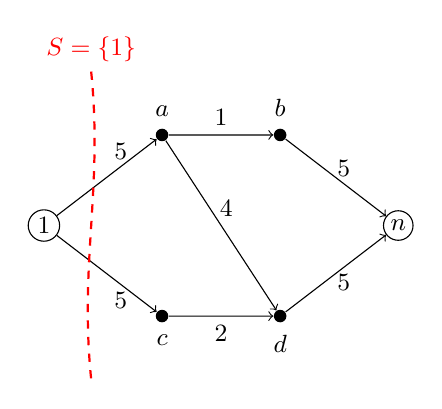
\begin{tikzpicture}[xscale=1.5, yscale=1.15]
    \node (s) at (0,0) [circle, draw, inner sep=1.4pt] {\small $1$};
    \node (a) at (1,1) [circle, fill, inner sep=1.6pt] {};
    \node (b) at (2,1) [circle, fill, inner sep=1.6pt] {};
    \node (c) at (1,-1) [circle, fill, inner sep=1.6pt] {};
    \node (d) at (2,-1) [circle, fill, inner sep=1.6pt] {};
    \node (t) at (3,0) [circle, draw, inner sep=1.4pt] {\small $n$};
    \node[anchor=south] at (1,1.1) {\small $a$};
    \node[anchor=south] at (2,1.1) {\small $b$};
    \node[anchor=north] at (1,-1.1) {\small $c$};
    \node[anchor=north] at (2,-1.1) {\small $d$};
    \draw[->] (s) -- (a) node[pos=0.72, above left=-3pt] {\small $5$};
    \draw[->] (a) -- (b) node[pos=0.5, above] {\small $1$};
    \draw[->] (b) -- (t) node[pos=0.5, above right=-3pt] {\small $5$};
    \draw[->] (s) -- (c) node[pos=0.72, below left=-3pt] {\small $5$};
    \draw[->] (c) -- (d) node[pos=0.5, below] {\small $2$};
    \draw[->] (d) -- (t) node[pos=0.5, below right=-3pt] {\small $5$};
    \draw[->] (a) -- (d) node[pos=0.4, right] {\small $4$};
    \draw[dashed, thick, color=red] (0.4,1.7) .. controls (0.5,0.4) and (0.3,-0.4) .. (0.4,-1.7);
    \node[anchor=south, color=red] at (0.4,1.7) {\small $S = \{1\}$};
\end{tikzpicture}
\end{center}

The following inequality is the easy half of the story: no flow can beat any cut.

\begin{proposition}
    Let $x$ be a feasible flow with value $\delta$, and let $(S, V\setminus S)$ be any cut with $1 \in S$ and $n \in V\setminus S$. Then $\delta \leq C(S)$.
\end{proposition}
\begin{proof}
    For $X, Y \subseteq V$ write $f_x(X,Y) = \sum_{(i,j)\in E,\, i\in X,\, j \in Y}x_{ij}$ for the total flow from $X$ to $Y$. Summing the conservation equations over $i \in S$, all terms vanish except the one at $i = 1$, so
    $$
    \delta = \sum_{i \in S}\left(\sum_{j\,:\,(i,j)\in E}x_{ij} - \sum_{j\,:\,(j,i)\in E}x_{ji}\right) = f_x(S, V) - f_x(V, S).
    $$
    Splitting $V$ as $S \cup (V\setminus S)$ in both terms, the $f_x(S,S)$ contributions cancel, leaving
    $$
    \delta = f_x(S, V\setminus S) - f_x(V\setminus S, S) \leq f_x(S, V\setminus S) \leq C(S),
    $$
    using $f_x(V\setminus S, S) \geq 0$ and $x_{ij} \leq c_{ij}$.
\end{proof}

The remarkable fact is that this bound is always attained: some cut is exactly as good as the best flow. This is a theorem of Ford and Fulkerson, and it is a beautiful example of strong duality in a combinatorial setting -- the maximum flow problem and the minimum cut problem are dual to each other.

\begin{definition}[Augmenting Path]
    Let $x$ be a feasible flow. A path $v_0, v_1, \dots, v_k$ in the \emph{undirected} sense -- so consecutive vertices are joined by an edge in one direction or the other -- is an \vocab{augmenting path} if
    \begin{itemize}
        \item $x_{v_iv_{i+1}} < c_{v_iv_{i+1}}$ for every edge traversed forwards, and
        \item $x_{v_{i+1}v_i} > 0$ for every edge traversed backwards.
    \end{itemize}
\end{definition}

The point is that along such a path we can increase the flow by some $\varepsilon > 0$ on the forward edges and decrease it by $\varepsilon$ on the backward edges, and conservation still holds at every intermediate vertex. So if there is an augmenting path from $1$ to $n$, the flow value can be increased and $x$ was not optimal.

\begin{center}
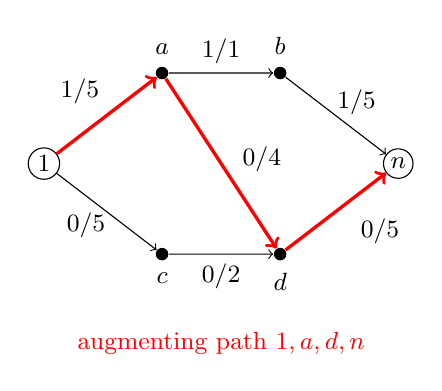
\begin{tikzpicture}[xscale=1.5, yscale=1.15]
    \node (s) at (0,0) [circle, draw, inner sep=1.4pt] {\small $1$};
    \node (a) at (1,1) [circle, fill, inner sep=1.6pt] {};
    \node (b) at (2,1) [circle, fill, inner sep=1.6pt] {};
    \node (c) at (1,-1) [circle, fill, inner sep=1.6pt] {};
    \node (d) at (2,-1) [circle, fill, inner sep=1.6pt] {};
    \node (t) at (3,0) [circle, draw, inner sep=1.4pt] {\small $n$};
    \node[anchor=south] at (1,1.1) {\small $a$};
    \node[anchor=south] at (2,1.1) {\small $b$};
    \node[anchor=north] at (1,-1.1) {\small $c$};
    \node[anchor=north] at (2,-1.1) {\small $d$};
    \draw[->, very thick, color=red] (s) -- (a);
    \draw[->, very thick, color=red] (a) -- (d);
    \draw[->, very thick, color=red] (d) -- (t);
    \draw[->] (a) -- (b) node[pos=0.5, above] {\small $1/1$};
    \draw[->] (b) -- (t) node[pos=0.5, above right=-3pt] {\small $1/5$};
    \draw[->] (s) -- (c) node[pos=0.5, below left=-3pt] {\small $0/5$};
    \draw[->] (c) -- (d) node[pos=0.5, below] {\small $0/2$};
    \node[anchor=south east] at (0.55,0.55) {\small $1/5$};
    \node[anchor=west] at (1.6,0.05) {\small $0/4$};
    \node[anchor=north west] at (2.6,-0.5) {\small $0/5$};
    \node[anchor=north, color=red] at (1.5,-1.75) {\small augmenting path $1,a,d,n$};
\end{tikzpicture}
\end{center}

\begin{theorem}[Max-Flow Min-Cut]
    The maximum value of a feasible flow equals the minimum capacity of a cut separating $1$ from $n$:
    $$
    \delta^* = \min\{C(S) : S \subseteq V,\ 1 \in S,\ n \in V\setminus S\}.
    $$
\end{theorem}
\begin{proof}
    By the proposition, $\delta^* \leq C(S)$ for every such cut, so it is enough to exhibit a cut with $C(S) = \delta^*$.

    Let $x$ be an optimal flow, and define
    $$
    S = \{1\}\cup\{i \in V : \text{ there is an augmenting path from } 1 \text{ to } i\}.
    $$
    Since $x$ is optimal there is no augmenting path from $1$ to $n$, so $n \notin S$ and $(S, V\setminus S)$ is a cut separating $1$ from $n$. From the proof of the proposition,
    $$
    \delta^* = f_x(S, V\setminus S) - f_x(V\setminus S, S),
    $$
    and we claim both terms take their extreme values.

    First, $f_x(V\setminus S, S) = 0$. Indeed, suppose $(v, u) \in E$ with $v \in V\setminus S$, $u \in S$ and $x_{vu} > 0$. Then we may extend an augmenting path from $1$ to $u$ by traversing $(v,u)$ backwards, obtaining an augmenting path from $1$ to $v$; so $v \in S$, a contradiction.

    Second, $f_x(S, V\setminus S) = C(S)$. Indeed, suppose $(u, v)\in E$ with $u \in S$, $v \in V\setminus S$ and $x_{uv} < c_{uv}$. Then we may extend an augmenting path from $1$ to $u$ by traversing $(u,v)$ forwards, so $v \in S$, again a contradiction. Hence every edge from $S$ to $V\setminus S$ is saturated.

    Therefore $\delta^* = C(S) - 0 = C(S)$, as required.
\end{proof}

Notice that the proof is constructive: it tells us that if we cannot find an augmenting path, we are done, and it even hands us the certifying cut. This is the algorithm.

\begin{definition}[Ford--Fulkerson Algorithm]
    To find a maximum flow:
    \begin{enumerate}[label=(\arabic*)]
        \item Start from any feasible flow, e.g.\ $x = 0$.
        \item Search for an augmenting path from $1$ to $n$. If there is none, stop -- $x$ is optimal.
        \item Increase the flow along the path by as much as possible (the smallest of $c_{ij} - x_{ij}$ over forward edges and $x_{ji}$ over backward edges), and go to (2).
    \end{enumerate}
\end{definition}

The bookkeeping is easiest with the \vocab{residual network}: for each edge $(i,j)$ we record a forward residual capacity $c_{ij} - x_{ij}$ and a backward residual capacity $x_{ij}$. An augmenting path is then just an ordinary directed path in the residual network, and the amount we can push is the smallest residual capacity along it.

\begin{center}
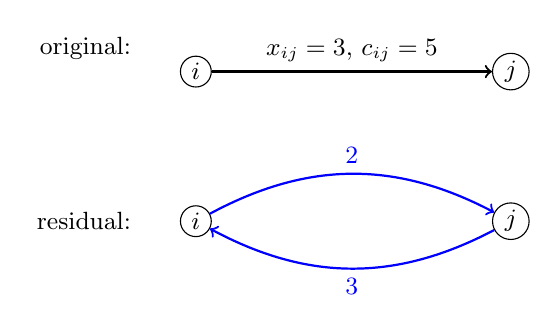
\begin{tikzpicture}[scale=1.0]
    \node[anchor=east] at (-0.7,0.3) {\small original:};
    \node (u) at (0,0) [circle, draw, inner sep=1.6pt] {\small $i$};
    \node (v) at (4.0,0) [circle, draw, inner sep=1.6pt] {\small $j$};
    \draw[->, thick] (u) -- (v) node[pos=0.5, above] {\small $x_{ij} = 3$, $c_{ij} = 5$};
    \begin{scope}[yshift=-1.9cm]
    \node[anchor=east] at (-0.7,0) {\small residual:};
    \node (u2) at (0,0) [circle, draw, inner sep=1.6pt] {\small $i$};
    \node (v2) at (4.0,0) [circle, draw, inner sep=1.6pt] {\small $j$};
    \draw[->, thick, color=blue] (u2) to[bend left=28] node[pos=0.5, above] {\small $2$} (v2);
    \draw[->, thick, color=blue] (v2) to[bend left=28] node[pos=0.5, below] {\small $3$} (u2);
    \end{scope}
\end{tikzpicture}
\end{center}

\begin{example}
    Consider the network drawn above, with capacities
    $$
    c_{1a} = 5,\quad c_{ab} = 1,\quad c_{bn} = 5,\quad c_{1c} = 5,\quad c_{cd} = 2,\quad c_{dn} = 5,\quad c_{ad} = 4,
    $$
    and start with $x = 0$.
    \begin{enumerate}[label=(\roman*)]
        \item The path $1, a, b, n$ is augmenting; the bottleneck is $c_{ab} = 1$, so we send $1$ unit. Now $x_{1a} = x_{ab} = x_{bn} = 1$ and $\delta = 1$.
        \item The path $1, a, d, n$ is augmenting; the bottleneck is $c_{1a} - x_{1a} = 4$, so we send $4$ units. Now $x_{1a} = 5$, $x_{ad} = 4$, $x_{dn} = 4$ and $\delta = 5$.
        \item The path $1, c, d, n$ is augmenting; the bottleneck is $c_{dn} - x_{dn} = 1$, so we send $1$ unit. Now $x_{1c} = x_{cd} = 1$, $x_{dn} = 5$ and $\delta = 6$.
    \end{enumerate}
    The final flow is $x_{1a} = 5$, $x_{ab} = 1$, $x_{bn} = 1$, $x_{ad} = 4$, $x_{1c} = 1$, $x_{cd} = 1$, $x_{dn} = 5$.

    To see that this is optimal we compute the set $S$ of vertices reachable from $1$ by an augmenting path. The edge $1a$ is saturated, so $a$ is not reachable that way; but $x_{1c} = 1 < 5$, so $c \in S$. From $c$, $x_{cd} = 1 < 2$, so $d \in S$. From $d$, the edge $dn$ is saturated, but the edge $ad$ carries flow $4 > 0$, so traversing it \emph{backwards} puts $a \in S$. From $a$, the edge $ab$ is saturated, so we get nothing new. Hence
    $$
    S = \{1, a, c, d\},
    $$
    and $n \notin S$, so this is a genuine cut. Its capacity is the total capacity of edges leaving $S$, namely $ab$ and $dn$:
    $$
    C(S) = c_{ab} + c_{dn} = 1 + 5 = 6 = \delta^*,
    $$
    confirming optimality.
\end{example}

\begin{remark}
    Finding the cut requires a little care: $S$ consists of everything reachable by an augmenting path, and augmenting paths may traverse edges backwards, so one must chase the reachability to the end. When Ford--Fulkerson stops, the set of reachable vertices is automatically a minimum cut -- that is exactly what the proof of the max-flow min-cut theorem showed.
\end{remark}

\begin{example}
    Here is a larger example in which a backward edge is genuinely needed. Take vertices $1, a, b, c, d, n$ with capacities
    $$
    c_{1a} = 10,\ c_{1c} = 10,\ c_{ab} = 4,\ c_{ac} = 2,\ c_{ad} = 8,\ c_{bn} = 10,\ c_{cd} = 9,\ c_{db} = 6,\ c_{dn} = 10,
    $$
    starting from $x = 0$.
    \begin{enumerate}[label=(\roman*)]
        \item Augment along $1, a, d, n$ by $\min(10, 8, 10) = 8$. Now $\delta = 8$, with $x_{1a} = 8$, $x_{ad} = 8$ (saturated) and $x_{dn} = 8$.
        \item Augment along $1, c, d, n$ by $\min(10, 9, 2) = 2$. Now $\delta = 10$, with $x_{1c} = 2$, $x_{cd} = 2$ and $x_{dn} = 10$ (saturated).
        \item Augment along $1, c, d, b, n$ by $\min(8, 7, 6, 10) = 6$. Now $\delta = 16$, with $x_{1c} = 8$, $x_{cd} = 8$, $x_{db} = 6$ (saturated) and $x_{bn} = 6$.
        \item Augment along $1, a, b, n$ by $\min(2, 4, 4) = 2$, the bottleneck being $c_{1a} - x_{1a} = 2$. Now $\delta = 18$, with $x_{1a} = 10$ (saturated), $x_{ab} = 2$ and $x_{bn} = 8$.
    \end{enumerate}
    At this stage the only unsaturated edge out of $1$ is $1c$, so $c \in S$; from $c$ we have $x_{cd} = 8 < 9$, so $d \in S$; from $d$ both $dn$ and $db$ are saturated, but $x_{ad} = 8 > 0$ so traversing $ad$ backwards gives $a \in S$; from $a$ we have $x_{ab} = 2 < 4$, so $b \in S$; and from $b$ we have $x_{bn} = 8 < 10$, so $n \in S$. So we have found an augmenting path,
    $$
    1 \rightarrow c \rightarrow d \xrightarrow{\ \text{backwards}\ } a \rightarrow b \rightarrow n,
    $$
    with bottleneck $\min(2, 1, 8, 2, 2) = 1$, coming from the edge $cd$. Augmenting by $1$ (and remembering to \emph{decrease} $x_{ad}$) gives $\delta = 19$ and
    $$
    x_{1a} = 10,\ x_{1c} = 9,\ x_{ab} = 3,\ x_{ac} = 0,\ x_{ad} = 7,\ x_{cd} = 9,\ x_{db} = 6,\ x_{bn} = 9,\ x_{dn} = 10.
    $$
    Now $1a$ is saturated and $x_{1c} = 9 < 10$, so $c \in S$; but from $c$ the edge $cd$ is saturated and the only other edge at $c$ is $ac$, which carries no flow. So $S = \{1, c\}$, and
    $$
    C(S) = c_{1a} + c_{cd} = 10 + 9 = 19 = \delta^*.
    $$
    So the flow of $19$ is optimal, certified by the cut $\{1, c\}$. Notice that without the backward step in the fifth augmentation we would have stopped at $\delta = 18$: the flow of $8$ units sent from $a$ to $d$ in step (i) was, with hindsight, a mistake, and the backward edge is precisely the mechanism by which the algorithm undoes it.
\end{example}

\begin{theorem}[Termination]
    If all capacities are integers, then the Ford--Fulkerson algorithm terminates in finitely many steps, and the maximum flow is integral.
\end{theorem}
\begin{proof}
    If $x$ is integral, then the bottleneck along any augmenting path is a positive integer, so the augmented flow is integral and the value increases by at least $1$. Since $\delta$ is bounded above by the capacity of any cut, only finitely many augmentations can occur. Starting from $x = 0$, which is integral, the result follows.
\end{proof}

The same argument works for rational capacities (clear denominators). For irrational capacities, the algorithm can in principle fail to terminate if the augmenting paths are chosen badly -- choosing shortest augmenting paths always works, and gives the Edmonds--Karp algorithm.

\subsection{An Application: Bipartite Matching}

The integrality in the theorem above is what makes max-flow such a powerful combinatorial tool: it turns questions about $\{0,1\}$-valued combinatorial objects into questions about flows.

\begin{theorem}
    Every $k$-regular bipartite graph has a perfect matching.
\end{theorem}
\begin{proof}
    Let $G$ be a bipartite graph with parts $L$ and $R$ each of size $N$, with every vertex having degree $k$. (The parts have equal size because counting edges gives $k|L| = |E| = k|R|$.) Build a flow network: add a source $1$ joined to every vertex of $L$ with capacity $1$, add a sink $n$ joined from every vertex of $R$ with capacity $1$, and direct every edge of $G$ from $L$ to $R$ with capacity $1$.

    The cut $S = \{1\}$ has capacity $N$, so $\delta^* \leq N$. On the other hand, sending $1/k$ along every edge of $G$ and $1$ along every edge from the source and to the sink gives a feasible flow of value $N$ (each vertex of $L$ receives $1$ and sends out $k \cdot \frac 1k = 1$). So $\delta^* = N$.

    By the previous theorem, since all capacities are integers, there is an \emph{integral} flow of value $N$. Every edge then carries flow $0$ or $1$, and every vertex of $L$ has exactly one outgoing edge with flow $1$ (it receives exactly $1$ from the source), and similarly every vertex of $R$ has exactly one incoming edge with flow $1$. The edges carrying flow $1$ therefore form a perfect matching.
\end{proof}

\begin{remark}
    The same technique proves Hall's marriage theorem: a bipartite graph with parts $L, R$ has a matching saturating $L$ if and only if $|N(A)| \geq |A|$ for every $A \subseteq L$. One shows that a cut of capacity less than $|L|$ in the network above corresponds exactly to a violating set $A$, and then applies max-flow min-cut.
\end{remark}

\section{Game Theory}

We close with a topic that at first sight has nothing to do with optimization: what should you do when the thing you are optimizing against is another person, who is optimizing against you? The answer, remarkably, is that a two-player zero-sum game is exactly a pair of dual linear programs, and the fundamental theorem of such games -- the minimax theorem -- is exactly strong duality. This is one of the most satisfying appearances of the theory we have built.

\subsection{Two-Player Zero-Sum Games}

\begin{definition}[Zero-Sum Game]
    A \vocab{two-person zero-sum game} consists of two players, $\mathrm{P}_1$ and $\mathrm{P}_2$, with $m$ and $n$ available actions respectively, and a \vocab{payoff matrix} $A \in \R^{m\times n}$. If $\mathrm{P}_1$ plays $i$ and $\mathrm{P}_2$ plays $j$, then $\mathrm{P}_1$ wins the amount $a_{ij}$ and $\mathrm{P}_2$ loses the same amount.
\end{definition}

So $\mathrm{P}_1$ chooses a row and wants the entry to be large; $\mathrm{P}_2$ chooses a column and wants it to be small. `Zero-sum' means that one player's gain is exactly the other's loss -- there is nothing to cooperate over.

Suppose first that the players move in sequence, and $\mathrm{P}_1$ must move first. If $\mathrm{P}_1$ plays row $i$ then $\mathrm{P}_2$, seeing this, will respond with the column minimizing $a_{ij}$. So $\mathrm{P}_1$ should solve
$$
\max_{i}\min_j a_{ij}.
$$
Symmetrically, if $\mathrm{P}_2$ moves first then $\mathrm{P}_2$ should solve
$$
\min_j\max_i a_{ij}.
$$
It is always the case that
$$
\max_i\min_j a_{ij} \leq \min_j\max_i a_{ij},
$$
since $\min_{j'}a_{ij'} \leq a_{ij} \leq \max_{i'}a_{i'j}$ for every $i, j$; taking the max over $i$ on the left and the min over $j$ on the right preserves this. Moving second is (weakly) an advantage: you get to see what your opponent did.

\begin{definition}[Saddle Point]
    An entry $a_{i^*j^*}$ is a \vocab{saddle point} if it is simultaneously the minimum of its row and the maximum of its column, that is
    $$
    a_{i^*j} \geq a_{i^*j^*} \geq a_{ij^*} \quad\text{ for all } i, j.
    $$
    Equivalently, $\max_i\min_j a_{ij} = a_{i^*j^*} = \min_j\max_i a_{ij}$. In this case $a_{i^*j^*}$ is called the \vocab{value} of the game.
\end{definition}

The name comes from the geometry: at a saddle point the payoff surface curves up in one direction and down in the other, like a mountain pass.

\begin{center}
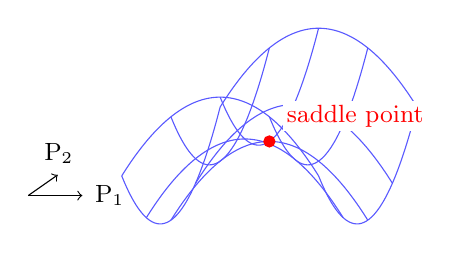
\begin{tikzpicture}[scale=1.25]
    % saddle surface: height h = -0.8 u^2 + 0.8 w^2, projected by (u,w) -> (u + 0.5w, 0.35w + h)
    % curves of constant w (varying u, the P1 direction): concave down
    \foreach \k in {-1,-0.5,0,0.5,1} {
        \draw[color=blue!65, thin, samples=40, smooth, domain=-1:1]
            plot ({\x + 0.5*\k}, {0.35*\k - 0.8*\x*\x + 0.8*\k*\k});
    }
    % curves of constant u (varying w, the P2 direction): concave up
    \foreach \k in {-1,-0.5,0,0.5,1} {
        \draw[color=blue!65, thin, samples=40, smooth, domain=-1:1]
            plot ({\k + 0.5*\x}, {0.35*\x - 0.8*\k*\k + 0.8*\x*\x});
    }
    \filldraw[color=red] (0,0) circle (1.6pt);
    \node[fill=white, inner sep=1.5pt, anchor=south west, text=red] at (0.13,0.1) {\small saddle point};
    \draw[->] (-2.45,-0.55) -- (-1.9,-0.55);
    \node[anchor=west] at (-1.87,-0.55) {\small $\mathrm{P}_1$};
    \draw[->] (-2.45,-0.55) -- (-2.15,-0.34);
    \node[anchor=south] at (-2.14,-0.32) {\small $\mathrm{P}_2$};
\end{tikzpicture}
\end{center}

\begin{example}
    Take
    $$
    A = \begin{pmatrix}1 & 2\\3&4\end{pmatrix}.
    $$
    Row minima are $1$ and $3$, so $\max_i\min_j a_{ij} = 3$. Column maxima are $3$ and $4$, so $\min_j\max_i a_{ij} = 3$. These agree, so $(2,1)$ is a saddle point and the value of the game is $3$. Both players should play their part of the saddle point regardless of who moves first, and neither can do better by deviating.
\end{example}

\begin{example}
    Take
    $$
    A = \begin{pmatrix}4 & 2\\1&3\end{pmatrix}.
    $$
    Row minima are $2$ and $1$, so $\max_i\min_j a_{ij} = 2$. Column maxima are $4$ and $3$, so $\min_j\max_i a_{ij} = 3$. These do not agree, and there is no saddle point.

    In this game there is no stable pair of choices. If $\mathrm{P}_1$ plays row $1$ then $\mathrm{P}_2$ prefers column $2$; but against column $2$, $\mathrm{P}_1$ prefers row $2$; against row $2$, $\mathrm{P}_2$ prefers column $1$; against column $1$, $\mathrm{P}_1$ prefers row $1$ -- and we are back where we started. Whatever either player does, if the other knows it they can exploit it.
\end{example}

\subsection{Mixed Strategies}

The resolution of the second example is one of the great ideas of game theory: the players should randomize. If $\mathrm{P}_1$ picks a row at random according to a probability distribution, then $\mathrm{P}_2$ cannot know which row will be played, only the distribution, and so cannot exploit the choice exactly.

\begin{definition}[Mixed Strategy]
    A \vocab{mixed strategy} for $\mathrm{P}_1$ is a vector $p \in \R^m$ with $p \geq 0$ and $\sum_i p_i = 1$, where $p_i$ is the probability of playing action $i$. Similarly a mixed strategy for $\mathrm{P}_2$ is $q \in \R^n$ with $q \geq 0$, $\sum_j q_j = 1$. A strategy which plays one action with probability $1$ is called \vocab{pure}.
\end{definition}

If $\mathrm{P}_1$ plays $p$ and $\mathrm{P}_2$ plays $q$, the expected payoff to $\mathrm{P}_1$ is
$$
\sum_{i,j}p_i a_{ij}q_j = p\cdot(Aq) = p^TAq.
$$
If $\mathrm{P}_1$ plays $p$ and $\mathrm{P}_2$ responds with a pure strategy $j$, the expected payoff is $\sum_i a_{ij}p_i = (A^Tp)_j$; and since a mixed strategy is an average of pure ones, $\mathrm{P}_2$ can do no better than the best pure response. So $\mathrm{P}_1$ wants to solve
\begin{alignat*}{2}
    & \text{maximize} \quad && \min_{j}\ (A^Tp)_j\\
    & \text{subject to} \quad && \textstyle\sum_i p_i = 1,\ p \geq 0.
\end{alignat*}
This is not yet a linear program, but the standard trick of introducing a variable for the minimum makes it one. Writing $e = (1,1,\dots,1)^T$ (of whatever length is needed),
\begin{alignat*}{2}
    (\mathrm{P}_1) \qquad & \text{maximize} \quad && v \\
    & \text{subject to} \quad && A^Tp \geq ve,\\
    & && e\cdot p = 1,\ p \geq 0.
\end{alignat*}
Similarly, $\mathrm{P}_2$ wants to minimize the maximum expected loss, giving
\begin{alignat*}{2}
    (\mathrm{P}_2) \qquad & \text{minimize} \quad && w \\
    & \text{subject to} \quad && Aq \leq we,\\
    & && e\cdot q = 1,\ q \geq 0.
\end{alignat*}
Both are honest linear programs, in the variables $(p, v)$ and $(q, w)$ respectively. And now the punchline.

\begin{theorem}
    The problems $(\mathrm{P}_1)$ and $(\mathrm{P}_2)$ are dual to each other.
\end{theorem}
\begin{proof}
    Introduce a slack variable $s \geq 0$ to write $\mathrm{P}_2$'s constraints as $Aq + s = we$, and take multipliers $\lambda_1 \in \R^m$ for these and $\lambda_2 \in \R$ for the normalization $e\cdot q = 1$. The Lagrangian is
    \begin{align*}
        L(w, q, s, \lambda) &= w + \lambda_1\cdot(Aq + s - we) - \lambda_2(e\cdot q - 1)\\
        &= w\left(1 - \lambda_1\cdot e\right) + \left(A^T\lambda_1 - \lambda_2 e\right)\cdot q + \lambda_1\cdot s + \lambda_2.
    \end{align*}
    Now: $w$ is unrestricted, so we need $\lambda_1\cdot e = 1$; $q \geq 0$, so we need $A^T\lambda_1 - \lambda_2 e \geq 0$; and $s \geq 0$, so we need $\lambda_1 \geq 0$. Given all of these the infimum is $\lambda_2$. Hence the dual problem is
    \begin{alignat*}{2}
        & \text{maximize} \quad && \lambda_2 \\
        & \text{subject to} \quad && A^T\lambda_1 \geq \lambda_2 e,\\
        & && e\cdot\lambda_1 = 1,\ \lambda_1 \geq 0,
    \end{alignat*}
    which is exactly $(\mathrm{P}_1)$ under the identification $\lambda_1 = p$, $\lambda_2 = v$.
\end{proof}

\begin{theorem}[Minimax Theorem]
    For any payoff matrix $A$,
    $$
    \max_{p}\min_{q}\ p^TAq = \min_{q}\max_{p}\ p^TAq,
    $$
    where the maximum and minimum are over mixed strategies. The common value $v$ is called the \vocab{value} of the game.
\end{theorem}
\begin{proof}
    The left-hand side is the optimal value of $(\mathrm{P}_1)$ and the right-hand side is the optimal value of $(\mathrm{P}_2)$, and we have just shown these are dual linear programs. Both are feasible -- take $p$ and $q$ uniform, and $v, w$ suitably extreme -- and both are bounded, since $\min_{i,j}a_{ij} \leq p^TAq \leq \max_{i,j}a_{ij}$ always. So strong duality applies and the optimal values agree.
\end{proof}

This is a genuinely surprising theorem. It says that in a zero-sum game, once we allow randomization, there is no advantage to moving second: $\mathrm{P}_1$ can guarantee an expected payoff of at least $v$ no matter what $\mathrm{P}_2$ does, and $\mathrm{P}_2$ can guarantee losing at most $v$ no matter what $\mathrm{P}_1$ does. The game has a well-defined value, and there is no secret to keep.

The complementary slackness conditions for this dual pair are worth recording, since they are what we use to compute.

\begin{theorem}[Optimality Conditions for Games]
    Mixed strategies $p, q$ are optimal for $\mathrm{P}_1$ and $\mathrm{P}_2$ respectively, with value $v$, if and only if
    \begin{enumerate}[label=(\roman*)]
        \item $A^Tp \geq ve$, $e\cdot p = 1$, $p \geq 0$; \hfill (primal feasibility)
        \item $Aq \leq ve$, $e\cdot q = 1$, $q \geq 0$; \hfill (dual feasibility)
        \item $v = p^TAq$. \hfill (complementary slackness)
    \end{enumerate}
\end{theorem}
\begin{proof}
    Complementary slackness for the dual pair above reads $p\cdot(Aq - we) = 0$ and $q\cdot(A^Tp - ve) = 0$. Since $e\cdot p = e\cdot q = 1$, these say $p^TAq = w$ and $p^TAq = v$ respectively, so at an optimum $v = w = p^TAq$.
\end{proof}

The practical content of (iii) is the following pair of statements, which we will use in a moment:
\begin{itemize}
    \item if $p_i > 0$ then the $i$th constraint of $\mathrm{P}_2$'s problem is tight, i.e.\ $(Aq)_i = v$;
    \item if $q_j > 0$ then the $j$th constraint of $\mathrm{P}_1$'s problem is tight, i.e.\ $(A^Tp)_j = v$.
\end{itemize}
In words: every action that a player actually uses with positive probability must give exactly the value of the game against the opponent's optimal strategy. If some action gave strictly less, the player would drop it.

\subsection{Finding Optimal Strategies}

In principle we can always solve the linear program by the simplex method, but for small games there are shortcuts.
\begin{enumerate}[label=(\arabic*)]
    \item \textbf{Look for a saddle point.} If the payoff matrix has one, the corresponding pure strategies are optimal for both players and we are done.
    \item \textbf{Eliminate dominated actions.} If $a_{ij} \geq a_{i'j}$ for every $j$, then row $i$ \vocab{dominates} row $i'$: $\mathrm{P}_1$ can never do worse by playing $i$ instead of $i'$, so there is an optimal strategy with $p_{i'} = 0$, and we may delete row $i'$. Similarly, if $a_{ij} \leq a_{ij'}$ for every $i$ then column $j$ dominates column $j'$ (from $\mathrm{P}_2$'s point of view, smaller is better), and we may delete column $j'$.
    \item \textbf{Reduce to a small linear program.} A $2 \times n$ or $m\times 2$ game reduces to a one-dimensional problem that can be solved graphically.
    \item \textbf{Use complementary slackness} to recover the other player's strategy once you have one of them.
\end{enumerate}

\begin{example}
    Let us return to the game with no saddle point,
    $$
    A = \begin{pmatrix} 4 & 2\\1&3\end{pmatrix},
    $$
    and solve it properly. Write $\mathrm{P}_1$'s mixed strategy as $p = (p, 1-p)$. Against $\mathrm{P}_2$'s two pure strategies the expected payoffs are
    $$
    (A^Tp)_1 = 4p + (1-p) = 1 + 3p, \qquad (A^Tp)_2 = 2p + 3(1-p) = 3 - p,
    $$
    and $\mathrm{P}_1$ wants to maximize the smaller of these. The first is increasing in $p$ and the second decreasing, so the maximum of the minimum is where they cross:
    $$
    1 + 3p = 3 - p \implies p = \tfrac12, \qquad v = \tfrac52.
    $$
    Similarly, writing $q = (q, 1-q)$ for $\mathrm{P}_2$,
    $$
    (Aq)_1 = 4q + 2(1-q) = 2 + 2q, \qquad (Aq)_2 = q + 3(1-q) = 3 - 2q,
    $$
    and $\mathrm{P}_2$ minimizes the larger of these, which happens where $2 + 2q = 3 - 2q$, that is $q = \frac14$, again with value $\frac52$.

    So the value of the game is $\frac52$, with $p^* = \left(\frac12,\frac12\right)$ and $q^* = \left(\frac14,\frac34\right)$. Notice that $\frac52$ lies strictly between $\max_i\min_j a_{ij} = 2$ and $\min_j\max_i a_{ij} = 3$: randomizing has genuinely bought $\mathrm{P}_1$ something over any pure strategy, and it has cost $\mathrm{P}_2$ less than any pure strategy would have.

    Notice also the structure of the answer: at the optimum, \emph{both} of $\mathrm{P}_2$'s pure strategies give $\mathrm{P}_1$ the same expected payoff. This is complementary slackness at work -- since $q_1, q_2 > 0$, both of $\mathrm{P}_1$'s constraints must be tight. Equivalently, $\mathrm{P}_1$ chooses $p$ precisely so as to make $\mathrm{P}_2$ indifferent between their options; if $\mathrm{P}_2$ were not indifferent, they would have a strictly better reply and could exploit $\mathrm{P}_1$.
\end{example}

\begin{example}
    Consider the game with payoff matrix
    $$
    A = \begin{pmatrix} 2 & 3 & 4\\ 3 & 1 & \frac12\\ 1 & 3 & 2\end{pmatrix}.
    $$
    First, is there a saddle point? The row minima are $2, \frac12, 1$, so $\max_i\min_j = 2$; the column maxima are $3, 3, 4$, so $\min_j\max_i = 3$. These differ, so there is no saddle point and we will need mixed strategies.

    Next, look for domination. Row $1$ is $(2,3,4)$ and row $3$ is $(1,3,2)$; since $2 \geq 1$, $3\geq 3$ and $4 \geq 2$, row $1$ dominates row $3$, so we may take $p_3 = 0$ and work with
    $$
    \tilde A = \begin{pmatrix}2 & 3 & 4\\3&1&\frac12\end{pmatrix}.
    $$
    Write $\mathrm{P}_1$'s strategy as $p = (p, 1-p, 0)$. Then $\mathrm{P}_1$'s problem becomes
    \begin{alignat*}{2}
        & \text{maximize} \quad && v \\
        & \text{subject to} \quad && 2p + 3(1-p) \geq v,\\
        & && 3p + 1(1-p) \geq v,\\
        & && 4p + \tfrac12(1-p) \geq v,\\
        & && 0 \leq p \leq 1,
    \end{alignat*}
    that is, $v \leq \min\left\{3 - p,\ 1 + 2p,\ \tfrac12 + \tfrac72 p\right\}$, and we want to choose $p$ to make this minimum as large as possible. Since this is a one-dimensional problem we can just draw the three lines and look at their lower envelope.

\begin{center}
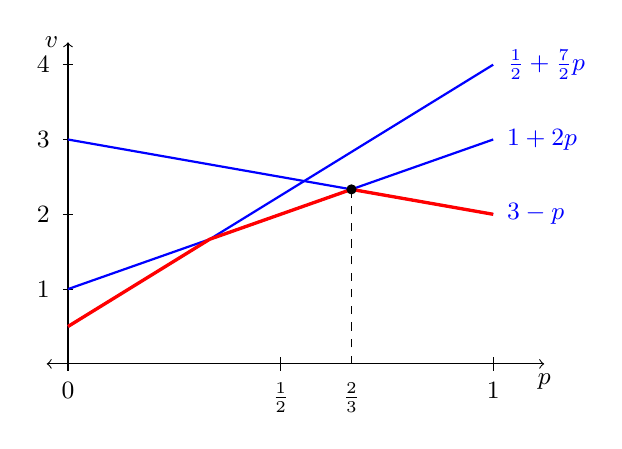
\begin{tikzpicture}[xscale=5.4, yscale=0.95]
    \draw[<->] (-0.05,0) -- (1.12,0) node[anchor=north] {\small $p$};
    \draw[->] (0,0) -- (0,4.3) node[anchor=east] {\small $v$};
    \foreach \p/\lab in {0/0, 0.5/{\frac12}, 1/1} {
        \draw (\p,-0.09) -- (\p,0.09);
        \node[anchor=north] at (\p,-0.12) {\small $\lab$};
    }
    \foreach \v in {1,2,3,4} {
        \draw (-0.012,\v) -- (0.012,\v);
        \node[anchor=east] at (-0.02,\v) {\small $\v$};
    }
    % 3 - p
    \draw[thick, color=blue] (0,3) -- (1,2);
    \node[anchor=west, color=blue] at (1.01,2) {\small $3 - p$};
    % 1 + 2p
    \draw[thick, color=blue] (0,1) -- (1,3);
    \node[anchor=west, color=blue] at (1.01,3) {\small $1 + 2p$};
    % 1/2 + 7/2 p
    \draw[thick, color=blue] (0,0.5) -- (1,4);
    \node[anchor=west, color=blue] at (1.01,4) {\small $\frac12 + \frac72 p$};
    % lower envelope highlighted
    \draw[very thick, color=red] (0,0.5) -- (0.3333,1.6667) -- (0.6667,2.3333) -- (1,2);
    \node[circle, fill, inner sep=1.3pt] at (0.6667,2.3333) {};
    \draw[dashed] (0.6667,0) -- (0.6667,2.3333);
    \node[anchor=north] at (0.6667,-0.12) {\small $\frac23$};
\end{tikzpicture}
\end{center}

    The lower envelope, drawn in red, is maximized where the lines $3 - p$ and $1 + 2p$ cross, at $p = \frac23$, giving $v = \frac73$. (The third line, $\frac12 + \frac72 p$, takes the value $\frac12 + \frac73 = \frac{17}{6} > \frac73$ there, so it is not binding.) So
    $$
    p^* = \left(\tfrac23, \tfrac13, 0\right), \qquad v = \tfrac73.
    $$
    Now we use complementary slackness to find $\mathrm{P}_2$'s strategy $q$. Since $p_1, p_2 > 0$, the first two constraints of $\mathrm{P}_2$'s problem must be tight:
    $$
    (Aq)_1 = 2q_1 + 3q_2 + 4q_3 = \tfrac73, \qquad (Aq)_2 = 3q_1 + q_2 + \tfrac12 q_3 = \tfrac73.
    $$
    Also, the third constraint of $\mathrm{P}_1$'s problem is slack (we computed $\frac{17}{6} > \frac73$), so complementary slackness forces $q_3 = 0$. With $q_1 + q_2 = 1$, the first equation gives
    $$
    2q_1 + 3(1 - q_1) = \tfrac73 \implies 3 - q_1 = \tfrac73 \implies q_1 = \tfrac23,
    $$
    and one checks that the second equation is satisfied: $3\cdot\frac23 + \frac13 = \frac73$. So
    $$
    q^* = \left(\tfrac23, \tfrac13, 0\right).
    $$
    Finally we should sanity check the answer against the optimality conditions. We have $A^Tp^* = \left(\frac73, \frac73, \frac{17}{6}\right) \geq \frac73 e$ and $Aq^* = \left(\frac73, \frac73, \frac53\right) \leq \frac73 e$, and $p^{*T}Aq^* = \frac73$. All three conditions hold, so $p^*$ and $q^*$ really are optimal and the value of the game is $\frac73$.
\end{example}

\begin{remark}
    It is worth noticing what this answer means. $\mathrm{P}_1$'s value from playing the pure strategy `always row $1$' is only $2$ (their opponent would always answer with column $1$), and from `always row $2$' is only $\frac12$. By mixing the two in the ratio $2:1$, $\mathrm{P}_1$ guarantees $\frac73 > 2$. Randomization is strictly better than any deterministic play. That this is possible at all, and that the resulting value is exactly matched by the opponent's best defence, is the content of the minimax theorem -- which is to say, of linear programming duality.
\end{remark}

